%% This is an example file to show how to use JASA_manu.sty and related 
%% files written by Eric C. Anderson.  It's sort of a fly-by-night endeavor,
%% but I got it to work for me!!

\documentclass[11pt]{article}

\usepackage{graphicx}
\usepackage{amsmath}
\usepackage{amssymb}
\usepackage{natbib}
\usepackage{JABES_manu}

% A few custom commands for bold-faced greek letters and regular letters
\def\balpha{\pmb{\alpha}}
\def\bbeta{\pmb{\beta}}
\def\bgamma{\pmb{\gamma}}
\def\bdelta{\pmb{\delta}}
\def\bmu{\pmb{\mu}}
\def\bsigma{\pmb{\sigma}}
\def\bSigma{\pmb{\Sigma}}
\def\bphi{\pmb{\phi}}
\def\bTheta{\pmb{\Theta}}
\def\btheta{\pmb{\theta}}
\def\btau{\pmb{\tau}}
\def\bomega{\pmb{\omega}}

\def\bX{\pmb{X}}
\def\bY{\pmb{Y}}
\def\bZ{\pmb{Z}}
\def\bJ{\pmb{J}}
\def\bV{\pmb{V}}
\def\bR{\pmb{R}}
\def\bW{\pmb{W}}
\def\bB{\pmb{B}}
\def\bA{\pmb{A}}



\begin{document}

\title{Hierarchical Bayes models for daily rainfall time series at multiple locations from heterogenous data sources}
\author{}

\maketitle

%% ABSTRACT
\newpage
\begin{center}
\textbf{Abstract}
\end{center}
We estimate a Hierarchical Bayesian models for daily rainfall that incorporates two novelties for estimating spatial and temporal correlations. We estimate the within site time series correlations for a particular rainfall site using multiple data sources at a given location, and we estimate the across site covariance in rainfall based on location distance. Previous rainfall models have captured cross site correlations as a functions of site specific distances, but not within site correlations across multiple data sources, and not both aspects simultaneously. Further, we incorporate information on the technology used (satellite versus rain gauge) in our estimations, which is also a novel addition. This methodology has far reaching applications in providing more accurate and complex weather insurance contracts based combining information from multiple data sources from a  single site,  a crucial improvement in the face of climate change. Secondly, the modeling extends to many other data contexts where multiple datasources exist for a given event or variable where both within and between series covariances can be estimated over time.

\vspace*{.3in}

\noindent\textsc{Keywords}: {Precipitation Models, Index Insurance, Spatio-Temporal Models}

\newpage

%%%%%%%%%%%%%%%%%%%%%%%%%%%%%%%%%%%%%%%
\section{Introduction}\label{sec:intro}
%%%%%%%%%%%%%%%%%%%%%%%%%%%%%%%%%%%%%%%

The ability to simulate a realistic time-series of daily rainfall is crucial in modeling climate impacts, particularly in locations with limited weather observations.   Simulated rainfall is widely used as an input into many end-user applications across agriculture, health, hydrology and ecology.  Weather generators, or simulators, are often used ``fill in'' missing observations, examine uncertainty or to investigate situations where historical records are not sufficiently long to include extreme events.   However, the current explosion of climate adaptation programs has substantially increased the practical demands placed on weather simulators, demands that often exceed the capabilities of state of the art.  

One particularly salient example is the increase in weather index insurance in developing countries for which payouts are based on rainfall deficits.  These projects have grown from a couple hundred farmers to tens of millions over the past decade \cite{Greatrex2015}.   The price of the insurance must cover the payouts.  Price is therefore is driven by the probability of a payout, which is driven by the probability of the rainfall deficits relevant to major crop losses. Naturally, insurance projects have relied heavily on rainfall models to drive insurance price calculations.  Because payout formulas are closely tied to specific rainfall features relevant to the crops insured, it is important for rainfall models to accurately characterize the relevant details for infrequent, tail events.  These rainfall features are often challenging for rainfall models, such as onset, inter-annual variability, consecutive dry days, climate teleconnections, and local spatial relationships. Because of these challenges, there are reports of initial applications of weather models leading to spurious results and unpredictable prices \cite{Giannini2009}.  As a result, insurance companies often include substantial increases in the insurance price to protect against their lack of confidence in the rainfall models \cite{Osgood2012}.

Perhaps a greater challenge is data poverty;  insurance projects must often be implemented where there are few historical ground based rainfall observations.  In some cases, networks of new gauges are installed, and in others, new satellite datasets are used.  These alternative datasets often provide a great deal of additional knowledge about rainfall patterns at the site of interest.  However, it is a non-trivial challenge to combine these multiple information sources, especially as satellites measure rainfall in a fundamentally different way to gauges, with different spatial statistics.  In addition, in order to use these new sources of information, statistics and probabilities must be informed by any information available for the long histories necessary to characterize the extreme tail events that drive large insurance payouts. Often the historical record is captured over a region, but not by any individual data source.  Typically, the data is in the form of a series of different rain gauges across the region in which only a subset of rain gauges are operational during different years or decades.

Projects such as insurance need tools that can utilize short histories of new gauges, as well as the overlapping experiences of historical gauges in the region while utilizing information from other sources, such as satellite estimates to provide the best distributions possible.  They also need to be able to condition on climate processes to quantify impacts of decadal processes, climate change, and ENSO \cite{Bell2013}.   This paper provides advances in methodology towards such a tool, based on a Hierarchical Bayesian approach.  Our model incorporates two novel aspects to simultaneously take into account site-specific correlations across multiple data-sources, plus cross-site spatial correlations.

%Place within weather generator research: markov, distributions, multiple sites, h bayes
There have been a myriad of published methodologies on stochastic weather generation, as comprehensively described in \cite{Wilks1999}, \cite{Sanso2000} and \cite{Verdin2015}.   We aim to give a brief overview to explain how our model fits in with weather generator literature.  The concept of probabilistically modeling weather has existed since the early 1900s, leading to the first statistical model of rainfall in \cite{Gabriel1962}.  These statistical models were formalized as stochastic weather generators, conceived as a parametric, two step process as proposed by \cite{Richardson1981}.  Daily rainfall occurrence was modeled as a Markov chain, then other weather variables including rainfall intensity were randomly sampled from a pre-specified distributions (typically Gamma for rainfall).   In recent years weather generator research has focused on four main areas: 1. Better capturing the rainfall occurrence and intensity distributions; 2. Incorporating spatial correlations to allow estimation at a point with little or no input data 3. Including multiple data sources and covariates; and 4. Increasing computational efficiency and tool development.  

To better capture rainfall distributions, rainfall intensity models in the ``standard'' parametric approach have moved from exponential \cite{Richardson1981}, to gamma \cite{Thom1958, Katz1977, Buishand1978, Coe1984, Wilks1992} and more recently to mixed gamma with generalized Pareto distributions \cite{Lennartsson2008}, or Weibull distributions \cite{Wilks1989, Furrer2008}.  More complex  Markov Chains have been suggested for rainfall occurrence \cite{Jones1993, Dastidar2010}, followed by recent research utilizing probit GLMs, allowing simulated temperatures to be better conditioned on rainfall occurrence \cite{Verdin2015}. Semi-parametric and non parametric approaches have also been devised, including a mix of Markov chains and re-sampling \cite{Apipattanavis2007}, semi-empirical histograms to model wet/dry spell length and rainfall intensity \cite{Racsko1991, Semenov2008} and fully non-parametric resampling \cite{Young1994,Lall1996, Rajagopalan1999}, or ensemble reordering \cite{Ghile2009}. In parallel to this research, new techniques have been utilized including Maximum Likelihood \cite{Fasso2011} and Bayes Theorem \cite{Sanso2000}.

Many of these techniques have allowed the incorporation of spatial information. \cite{Jones1993} used third order splines to interpolate their input parameters to locations with no observations. \cite{Wilks1998} incorporated spatial correlations into a Richardson weather generator by driving it with a grid of spatially correlated random numbers, followed by \cite{Baigorria2010} who developed this approach through the use of correlation matrices and orthogonal Markov chains.  \cite{Kleiber2012} utilized latent Gaussian processes to model spatial occurrence and rainfall amounts, an approach further extended in \cite{Kleiber2012} and \cite{Verdin2015} to include other variables. The approaches above would allow spatial correlations of statistics, but individual pixels-ensemble members would still remain independent. To overcome this issue, \cite{Greatrex2012} proposed utilizing the geostatistical technique of sequential simulation to create stochastically generated, spatially correlated maps of rainfall. 

There has been less research on the incorporation of multiple datasets. \cite{Furrer2008} incorporated ENSO into a rainfall generator via the use of GLMs. \cite{Fasso2011} used Maximum Likelihood Estimation to model heterogeneous environmental data, albeit to model air quality from satellite and ground based datasets, rather than to model rainfall. \cite{Hauser2013} utilized a Hidden Markov model linked with either polynomial regression or an artificial neural network to model rainfall conditioned on sea surface temperatures in the sub-polar North Atlantic.  This approach was also used by \cite{CareySmith2014} to incorporate varying seasonality into a Richardson weather generator.  In non-parametric research, \cite{Srivastav2015} used a maximum entropy bootstrap to simulate daily weather data in Canada.   To our knowledge, there has been no published research on the incorporation of multiple within-site realizations of rainfall, for example from gauges and satellites. 

Hierarchical bayesian estimation is yet another approach equipped to model spatial as well as temporal relationships.  These model and estimates the functional relationship between weather series over time. This was first proposed in \cite{Sans2015}, then extended by \cite{Sanso2000} to incorporate 1) spatial correlation for the joint distribution of weather series from several stations and 2) the non-stationarity of rainfall data. The authors show that their model is able to simulate weather data and summary statistics for a large number of stations, some of which have poor quality data. \cite{Lima2015} extended the methodology to model multi-site daily rainfall occurrence in order to investigate the distribution of the rainy season in Brazil.   

The aim of this paper is to present an extension of the Hierarchical Bayes approach to incorporate two new novelties. While we do not focus on the aspect of non-stationarity aspect in rainfall series, the novelty of our approach is our ability to account for two levels of the rainfall time series information at each site: 1) both the location of the measurement and 2) the instrument used to measure rainfall are incorporated. In addition, we 3) estimate the the spatial covariance between all these series and 4) the noise or error in recording rainfall due to the instrument itself. By incorporating several layers of information sources for each site in which we would like to predict weather, we are adding more information to the parameter estimates and, hopefully, improving out-of-sample predictions. Because we used daily data to fit our model, our simulated data and out-of-sample predictions are daily, which allows us to compute statistics sensitive to daily measurements: probability of rainfall, dry spells, and extreme rainfall.  We focus on a case study in a data-sparse region, the Tigray region of Ethiopia.


%The remainder the paper is as follows. In Section~\ref{sec:data} describes the data used and its preparation. In Section~\ref{sec:model} shows how rainfall the and the processes are modeled in a  hierarchical fashion. In Section~\ref{sec:fit} discusses the parameters to be estimated. Section~\ref{sec:sim} exhibits the performance in recovering parameters with simulated data. Section~\ref{sec:results} we graph the posteriors distributions for select parameters using the full historical data set. Section ~\ref{sec:metrics} exhibits some harder to estimate higher level rainfall metrics that practitioners would be interested in using: internal rainfall variability, probability of consecutive dry days, and probability of rainfall onset. Section~\ref{sec:discuss} concludes and describes next steps. 

%%%%%%%%%%%%%%%%%%%%%%%%%%%%%%
\section{Data}\label{sec:data}
%%%%%%%%%%%%%%%%%%%%%%%%%%%%%%

We model a set of 15 time series of daily rainfall in Ethiopia during the time period from 1992 to 2010, where these 15 time series come from six different locations, and each location has at least two time series of daily rainfall associated with it. The reason we observed multiple time series for each location is that for each location we have multiple sources of data, including rain station data and satellite-based rainfall proxy data. The statistical challenge to modeling such data is to separately estimate the spatial variability between locations and the within-location measurement-based variability. A standard hierarchical model with sets of 15 exchangeable parameters -- one for each time series -- would conflate these two sources of variation. The model we introduce here -- a hierarchical Bayesian model with one level for locations, and another level for multiple data sources within a location -- explicitly models each of these two sources of variation.

Figure~\ref{fig_ethiopia_map} shows the six locations from which the daily rainfall time series are measured. The names of the locations are Hagere Selam, Maykental, Mekele, Abi Adi, Agibe, and Adi Ha. The last of these, Adi Ha, is the location we are most interested in, because we wish to provide rainfall insurance for farmers who live there. Specifically, we want to model rainfall at one of the automated rain stations at Adi Ha, which is one of the 15 time series in our data set, but is also the series that has the least amount of observed data -- only about 200 days worth of data from 2009.

\begin{figure}[htbp]
\begin{center}
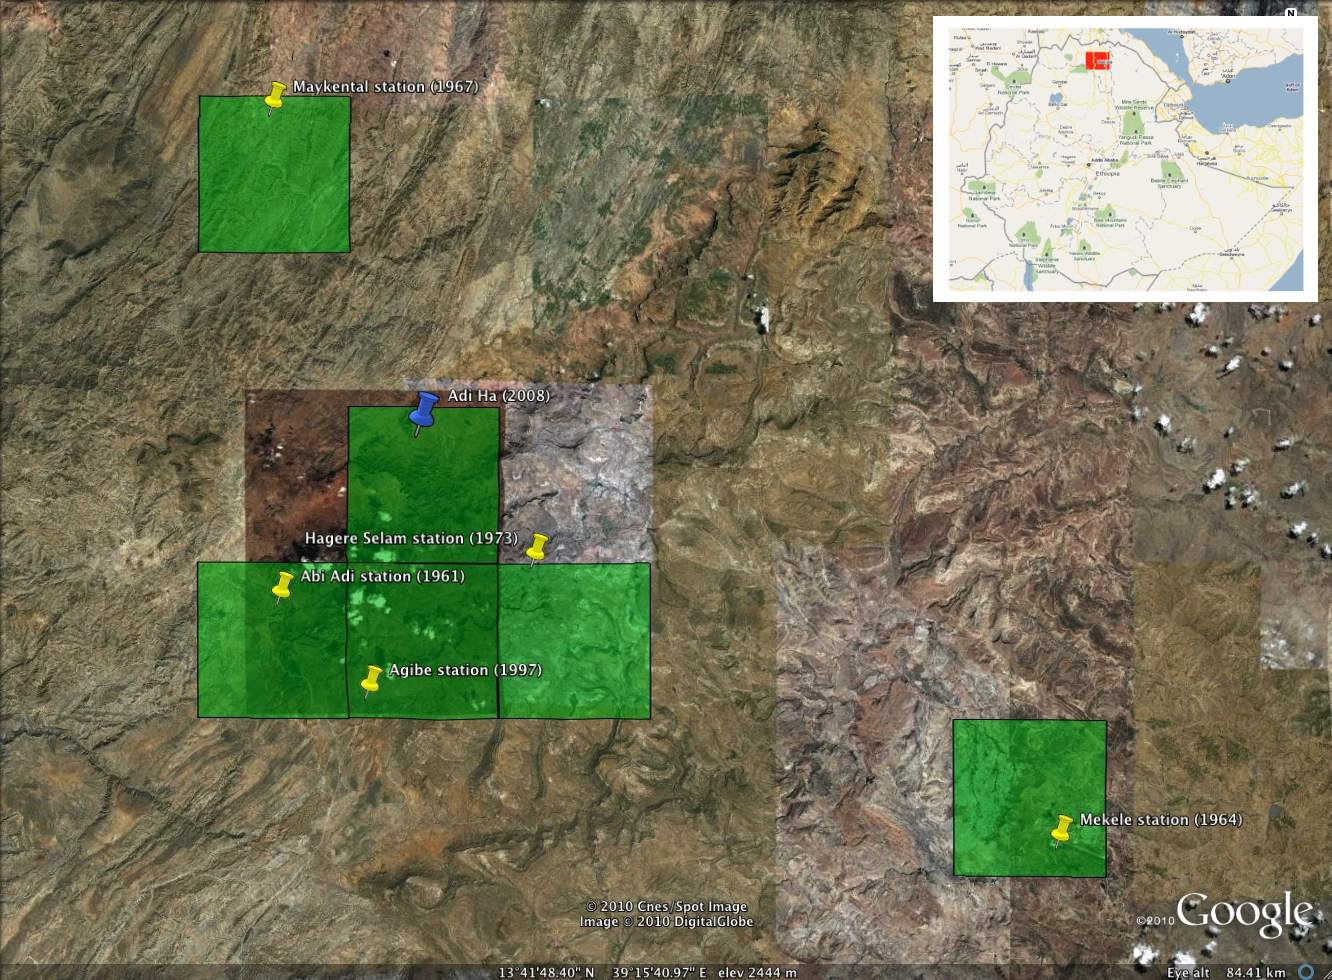
\includegraphics[width=4.5in]{fig_ethiopia_papermap.jpg}
\caption{A map of the 6 locations, where the green squares denote ARC pixels and the pins denote rain station locations. The inset in the upper right corner shows the area of the map with a red rectangular box; this region is in north central Ethiopia.}
\label{fig_ethiopia_map}
\end{center}
\end{figure}


The specifics of the data are as follows:
\begin{itemize}
\item For the first five locations, we have rain station data as well daily measurements from a satellite product called ARC, which is a rainfall proxy based on the temperature of the clouds over an area of about one hundred square kilometers. This comprises $ 5 \times 2 = 10$ time series.
\item For the sixth location, Adi Ha, we have five separate data sources:
\begin{enumerate}
\item One reliable rain station from which we only have 200 days of data from 2009-2010; this is the time series in which we have the most interest, because it is a new, accurate rain station on which we want to base insurance contracts.
\item One unreliable rain station from which we have about 7 years of data from 2000-2009, with about 2 years of missing data interspersed.
\item The ARC satellite proxy.
\item Two additional satellite proxies that are different from ARC.
\end{enumerate}
\end{itemize}

Figure~\ref{fig_overlap} shows the range of observed and missing data for each of these 15 time series; note that the time scale goes back to 1961 for one of the rain stations, but for simplicity, we only consider the time span of 1992-2010 in our model fit, because this span contains most of the data.

\begin{figure}[htbp]
\begin{center}
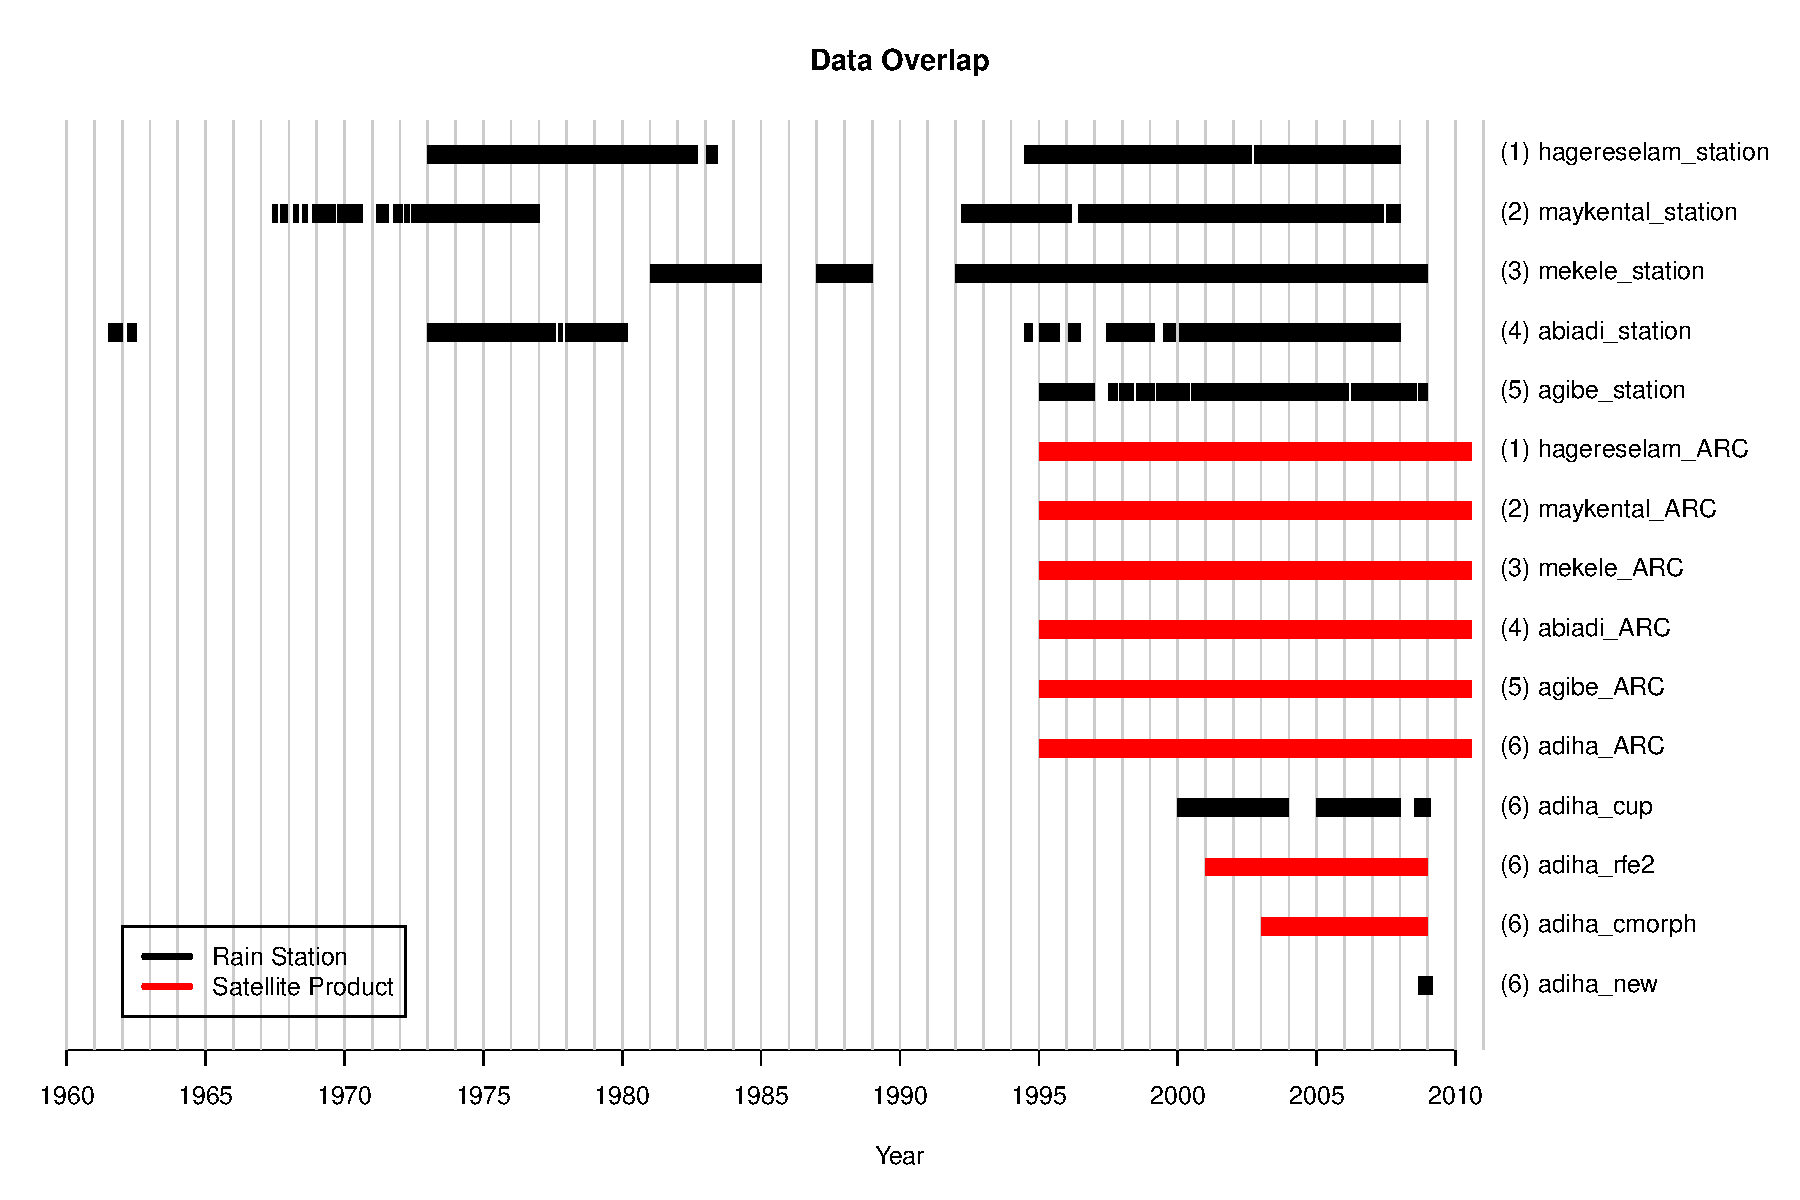
\includegraphics[width=5.0in]{fig_observed_data_new.pdf}
\caption{A visualization of the observed data for each of the 15 time series we model. The black hash marks denote rain station data, and the red hash marks denote satellite-based data.}
\label{fig_overlap}
\end{center}
\end{figure}


Table~\ref{tab_summary} contains some background information and summary statistics related to each time series of daily rainfall. For each time series we record the latitude, longitude, and elevation of the location where measurements were made, and the number of days of observed data. The maximum distance between locations is about 70 kilometers (between Mekele in the southeast and Maykental in the northwest).
\begin{table}[htdp]
\caption{Background information about the 15 time series}
\begin{center}
\begin{tabular}{|l|l|l|l|r|r|}
\hline
 & Site & Latitude & Longitude & Elev. (m) & Num. Obs \\
\hline
1 & Hagere Salaam & $13^\circ$ 38' 49'' & $39^\circ$ 10' 19'' & 2625 & 4887 \\
2 & Hagere Salaam (ARC) & '' & '' & '' & 5632 \\
3 & Maykental & $13^\circ$ 56' 13'' & $38^\circ$ 59' 49'' & 1819 & 5620 \\
4 & Maykental (ARC) & '' & '' & '' & 5632 \\
5 & Mekele & $13^\circ$ 28' 1'' & $39^\circ$ 31' 1'' & 2247 & 6205 \\
6 & Mekele (ARC) & '' & '' & '' & 5632 \\
7 & Abi Adi & $13^\circ$ 37' 19'' & $39^\circ$ 0' 10'' & 1849 & 4205 \\
8 & Abi Adi (ARC) & '' & '' & '' & 5632 \\
9 & Agibe & $13^\circ$ 33' 43'' & $39^\circ$ 3' 43'' & 1952 & 4722 \\
10 & Agibe (ARC) & '' & '' & '' & 5632 \\
11 & Adi Ha (ARC) & $13^\circ$ 43' 48'' & $39^\circ$ 05' 38'' & 1713 & 5632 \\
12 & Adi Ha (Rain Station - Manual) & '' & '' & '' & 2769 \\
13 & Adi Ha (RFE2) & '' & '' & '' & 2920 \\
14 & Adi Ha (CMorph) & '' & '' & '' & 2190 \\
15 & Adi Ha (Rain Station - Automatic) & '' & '' & '' & 186 \\
\hline
\end{tabular}
\end{center}
\label{tab_summary}
\end{table}

In this part of Ethiopia, the rainy season lasts roughly from June to October. Figure~\ref{fig_eda} shows the percentage of rainy days and the average amount of rain as a function of the time of year for each time series. The basic modeling strategy will be to use a set of periodic functions to model rainfall as a function of the season of the year.
\begin{figure}[ht]
\begin{center}
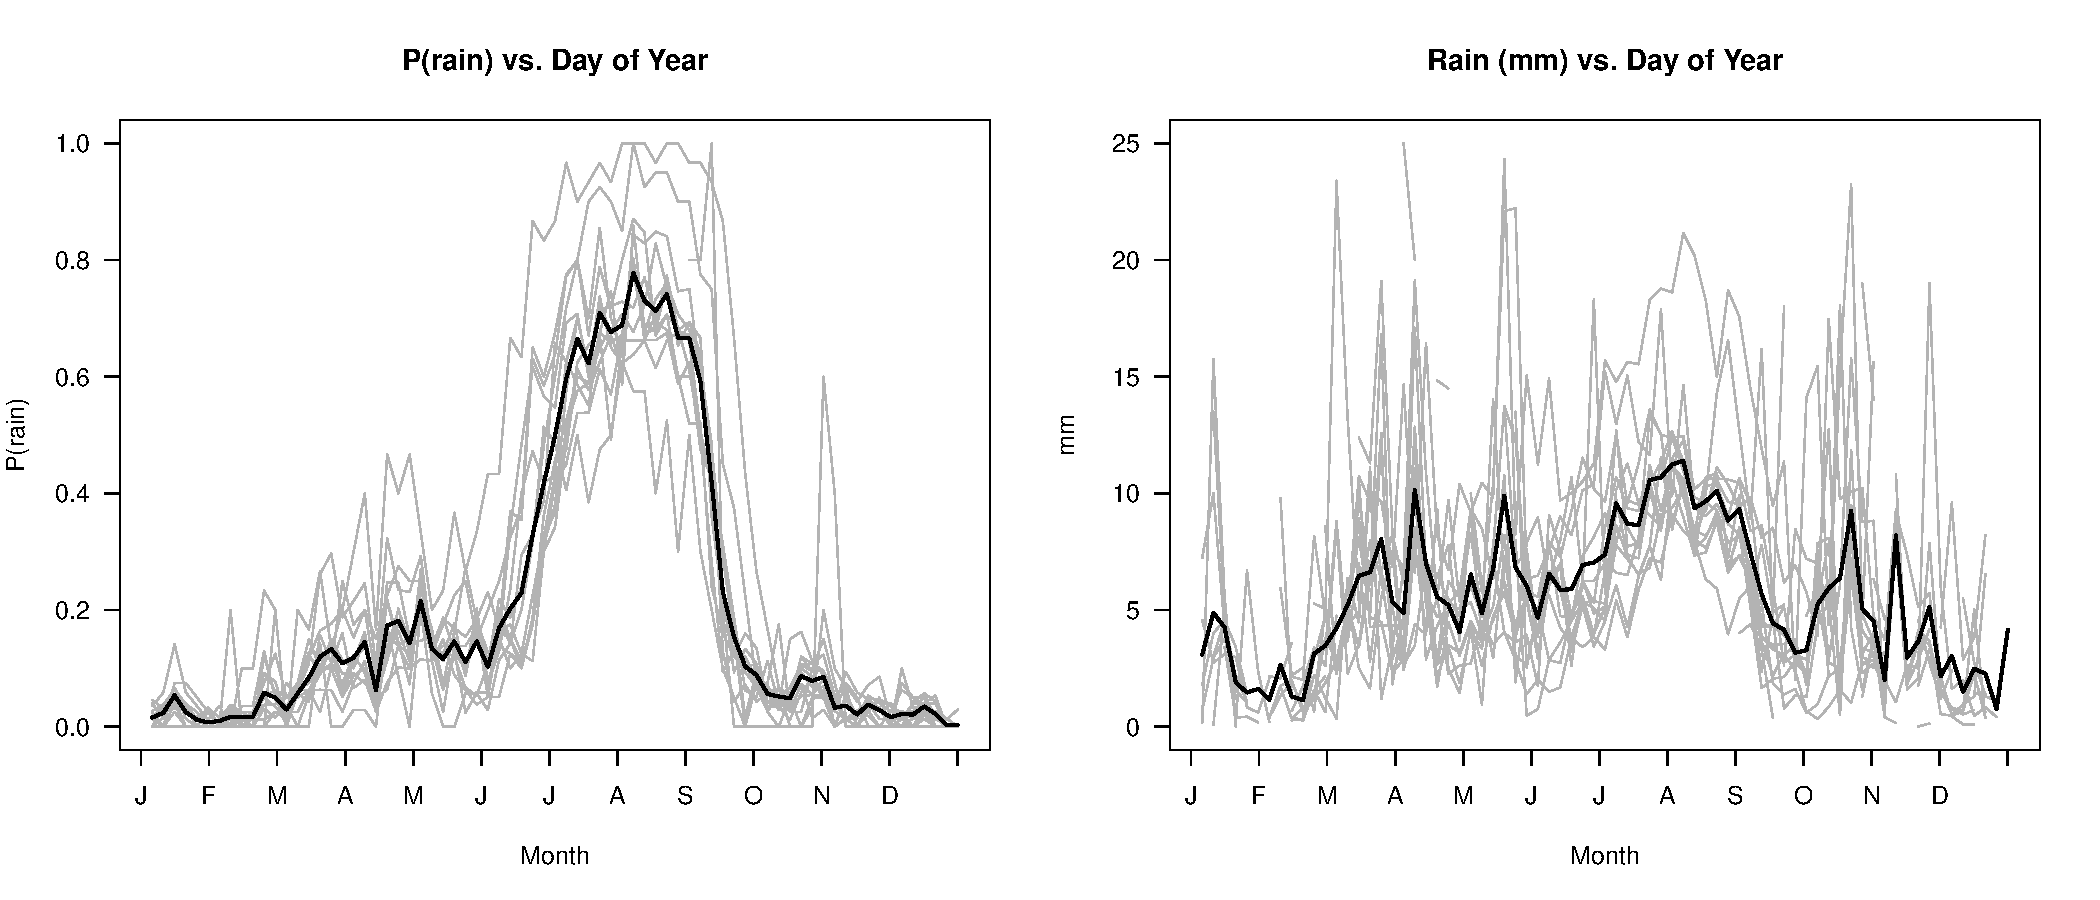
\includegraphics[width=6.5in]{fig_eda.pdf}
\caption{Plots of the percentage of rainy days (pooled into 5-day bins) and the average amount of rain as a function of the season. The gray lines are for each of the 15 individual time series, and the black lines are averaged across all 15 time series.}
\label{fig_eda}
\end{center}
\end{figure}

We are also interested in the difference, on average, between the measurements of rainfall based on the ARC satellite proxy and the rain stations. Comparing rainfall frequencies pooled over 5-day periods, averaging across all parts of the year and all five locations with exactly one rain station and one ARC measurement, we find that the ARC records about 3\% fewer days of rainfall than the rain stations. Across locations, this difference ranges from about -6\% (Hager Selam) to  +1\% (Agibe).



%%%%%%%%%%%%%%%%%%%%%%%%%%%%%%%%%%%%
\section{The Model}\label{sec:model}
%%%%%%%%%%%%%%%%%%%%%%%%%%%%%%%%%%%%
We fit a tobit model for daily rainfall at multiple locations, with multiple time series observed at each site. Let us first set up some notation. Let $S=6$ denote the number of locations where we measure rainfall, and $\bJ = \{2,2,2,2,2,5\}$ is the vector denoting the number of daily rainfall time series observed for each of the $S$ locations. The total number of days in our time series is $N=6679$ days, from 1/1/1992 through 7/28/2010. Let $Y_{stj}$ denote the amount of rainfall, measured in mm, for location $s \in (1,...,S)$, day $t \in (1,...,N)$, and time series $j = (1,...,J_s)$. Last, let $d_{ik}$ denote the Euclidian distance between site $i$ and $k$, for $i,k \in (1,...,S)$ in kilometers $\times$ 100.

We model $Y_{stj}$ using a hierarchical Bayesian tobit regression model, as specified below:
%, where the levels of the hierarchy correspond to different sources of variation

\newpage

% observations:
$\hspace{0.5in}
Y_{stj} = \begin{cases} W_{stj} &\mbox{if } W_{stj} > 0 \hspace{2.6in} \text{(1) Observed rainfall}\\
0  &\mbox{if } W_{stj} \leq 0, \end{cases}\\
$

% Latent continuous rainfall
$\hspace{0.9in}
\bW_{st} \sim \text{N}_{J_s}(\mathbf{1}Z_{st} + \bX^\text{ARC}_s \beta^\text{ARC}_s, \frac{1}{\gamma_{st}}\bSigma_s), \hspace{1.65in} \text{(2) Latent rainfall}
$

% Underlying spatial mean rainfall process for each location:
$\hspace{1.3in}
\bZ_t \sim N_S(\bX_t \bbeta^Z, \tau^2\bV), \hspace{1.85in} \text{(3) Spatial mean rainfall}
$

% seasonal effects
$\hspace{1.7in}
\beta_{ps}^Z \sim \text{N}(\mu_p, \sigma^2_p), \hspace{2.3in} \text{for } p = 1, 2, ..., 23
$

% mean of the groups of coefficients across locations
$\hspace{2.1in}
\mu_{p} \mid \sigma_p^2 \sim \text{N}(\mu_0, \sigma_p^2/\kappa_0),
$

% variance of the groups of coefficients across locations
$\hspace{2.4in}
%\sigma_{p} \sim \frac{1}{2}\text{t}(0, 1, \text{df} = 3),
\sigma_{p}^2 \sim \text{Inv-}\chi^2(v_0, \sigma_0^2),
$

% 'nugget effect' of spatial covariance:
$\hspace{1.7in}
%\tau \sim \frac{1}{2}\text{t}(0, 1, \text{df} = 3),
\tau \sim \text{Inv-Gamma}(\text{shape = } a_\tau, \text{scale = } b_\tau),
$

% parametric spatial covariance matrix, exponential model
$\hspace{1.7in}
\bV=\{v_{ik}\}, v_{ii}=1, v_{ik} = \exp(-\lambda d_{ik}),% \hspace{1.0in} \text{for $i,k \in (1,..,S)$}
$

% lambda determines the rate of spatial covariance decay across distance
$\hspace{2.1in}
\lambda \sim \text{gamma}(\text{shape} = a_\lambda, \text{ scale} = b_\lambda),
$

% X_t covariates
\vspace{-0.4in}
\begin{align*}
\hspace{1.2in}
\bX_t &= (1, t, t^2, \sin(2\pi t \omega_1), \cos(2\pi t \omega_1),..., \sin(2\pi t \omega_4), \cos(2\pi t \omega_4), \\
& \hspace{0.3in} X^\text{nino}_{\text{Jan}_{[t]}}, X^\text{nino}_{\text{Feb}_{[t]}}, ..., X^\text{nino}_{\text{Dec}_{[t]}}),
\end{align*}

\vspace{-0.2in}
% Indicator of ARC product
$\hspace{1.3in}
X^\text{ARC}_{sj} = 1(\text{jth time series at site s is an ARC product}),
$

% ARC effect:
$\hspace{1.3in}
\beta^\text{ARC}_s \sim \text{N}(\mu^\text{ARC}, \tau^2_\text{ARC}),
$

% mean ARC effect across locations
$\hspace{1.7in}
\mu^\text{ARC} \mid \tau_\text{ARC}^2 \sim \text{N}(\mu^\text{ARC}_0, \tau_\text{ARC}^2/\kappa_o^\text{ARC}),
$

% variance of ARC effects across locations:
$\hspace{2.18in}
\tau_\text{ARC}^2 \sim \text{Inv-}\chi^2(v_0^\text{ARC}, \sigma_0^{2^\text{ARC}}),
$

% Covariance matrices for each location:
$\hspace{1.3in}
\bSigma_s \sim \text{Inv-Wishart}(v_0 = J_s, \Lambda_0^{-1} = \text{diag}(J_s))
$

% mixture weight for normal covariances, resulting in multivariate t:
$\hspace{1.3in}
\gamma_{st} \sim \text{gamma}(\text{shape = } \frac{\alpha}{2}, \text{ scale = } \frac{2}{\alpha}),
$ \\
where $\mathbf{1}$ denotes the length-$J_s$ vector of ones for location $s = 1, .., S$. We set the values of the following hyperparameters, based on exploratory analysis, to be weakly informative prior distributions for their respective parameters (specifically, we used the method of moments to compute hyperparameter values that result in a prior with the desired mean and variance):
\begin{align}
& \mu_0 = 0; \kappa_0 = 1; v_0 = 5; \sigma_0^2 = 3/5, \\
& a_\tau = 12; b_\tau = 110 \\
& \mu_0^\text{ARC} = 0; \kappa_0^\text{ARC} = 1; v_0^\text{ARC} = 5; \sigma_0^{2^\text{ARC}} = 3/5, \\
& a_\lambda = 50; b_\lambda = 0.03, \\
& \alpha = 5.
\end{align}



\newpage

The explanation of the model is as follows.
\begin{enumerate}
\item The first level of the model is a standard tobit regression, where we model the observed rainfall, $Y_{stj}$, as being equal to the $j^{th}$ component of the latent rainfall vector, $\bW_{st}$, if it is greater than zero, and equal to zero if the $j^{th}$ component of the latent rainfall vector is less than or equal to zero.
\item Next, for each location $s$, the length-$J_s$ vector of latent rainfall amounts on day $t$, $\bW_{st}$, is a multivariate $t$ random variable centered at the spatial mean rainfall amount for that location and day, $Z_{st}$, and offset by an ARC bias effect, $\beta_s^\text{ARC}$ (where $X^\text{ARC}_{sj}$ is an indicator variable of whether time series $j$ at location $s$ is an ARC satellite product). The latent rainfall, $\bW_{st}$, is a multivariate-$t$ random variable because it is a scale mixture of multivariate normals with a mixture weight, $\frac{1}{\gamma_{st}}$, for the covariance, $\Sigma_s$, that is drawn from a gamma distribution.
\item The location-specific covariance matrices $\bSigma_s$ allow the multiple time series at each location to be correlated in unique ways. The mixing parameters $\gamma_{st}$ determine the widths of the tails of the multivariate-$t$ distributions, and are modeled with a gamma prior distribution with shape and scale parameters equal to 5/2 and 2/5, respectively, which implies that the multivariate-$t$ distribution, $\bW_{st}$, has 5 degrees of freedom. (In follow-up models, we could relax this assumption and estimate from the data how heavy the tails should be; the choice of 5 degrees of freedom is based on the fits of some simple, exploratory models).
\item The spatial mean rainfall amount for day $t$, $\bZ_t$, is modeled as a multivariate normal random variable whose mean depends on the day, $t$ (linearly, quadratically, and periodically, with periods $\bomega = \frac{1}{365}(1, 2, 3, 4)$), and also on effects from El Nino, where the El Nino effect is an additive constant that depends on the month (allowing El Nino to have different effects across the 12 months of the year).
\item The covariance matrix of $\bZ_t$, $\tau^2\bV$, depends on $\tau$, a scaling factor, one known input, the Euclidean distance between locations, and one unknown parameter, $\lambda$. The spatial correlation in rainfall between locations is modeled separately from the noise inherent in the different measurement methods at each location, which is modeled by $\bSigma_s$ for each location $s = 1, ..., S$. The model assumes that the covariances of pairs of $Z_{st}$'s decay exponentially with the Euclidian distance between the pairs of locations at the unknown rate $\lambda$, which we estimate from the data using a relatively flat prior.
\item The rest of the model is straightforward. We shrink the $\beta_{ps}^Z$'s for each location toward a common mean $\mu_p$. We also model the ARC biases, $\beta^\text{ARC}_s$ as normal random variables with an unknown mean, $\mu_\text{ARC}$, and variance $\tau_\text{ARC}^2$.
\end{enumerate}



%%%%%%%%%%%%%%%%%%%%%%%%%%%%%%%%%%%%%%%%%%
\section{Fitting the Model}\label{sec:fit}
%%%%%%%%%%%%%%%%%%%%%%%%%%%%%%%%%%%%%%%%%%

We sample from the joint posterior distribution of the parameters using an MCMC algorithm whose full details are specified in the Appendix. For each iteration, each step was a draw from the full conditional distribution of one of the parameters, except for the draw of $\lambda$, which was accomplished using a random-walk Metropolis step.

We ran the MCMC algorithm for 20,000 iterations in total, using the first 2,000 iterations as an adaptation period to tune the standard deviation of the proposal distribution for $\lambda$. 


\section{Simulation Study}
\label{sec:sim}
We first ran a simulation study, where we simulated data from a set of known parameters. These parameter values were chosen to approximate values that could have produced our observed data, based on EDA. The size of the simulated data set was similar to the real data in both dimensions (the number of time series and the number of days). We find that our model performs well with simulated data, in which are able to recover know parameters--in particular, our parameter for across and within site correlation. We were able to precisely estimate the spatial correlation between locations as well as the variability of different data sources within single locations. Below we show trace plots for parameters that are lower in the hierarchical model and thus more difficult to estimate, but also the primary contribution of this model. This includes: $\lambda$, $\tau^{ARC}$, and $\Sigma$. All three parameters were well-estimated, and convergence was relatively quick with a burn-in period of less than 5,000 draws. All other parameters were also well estimated and available upon request. 


%\begin{figure}[htbp]
%\begin{center}
%\caption{Simulation study results for $\lambda$ where the horizontal blue lines represent the known true values of the parameters.}
%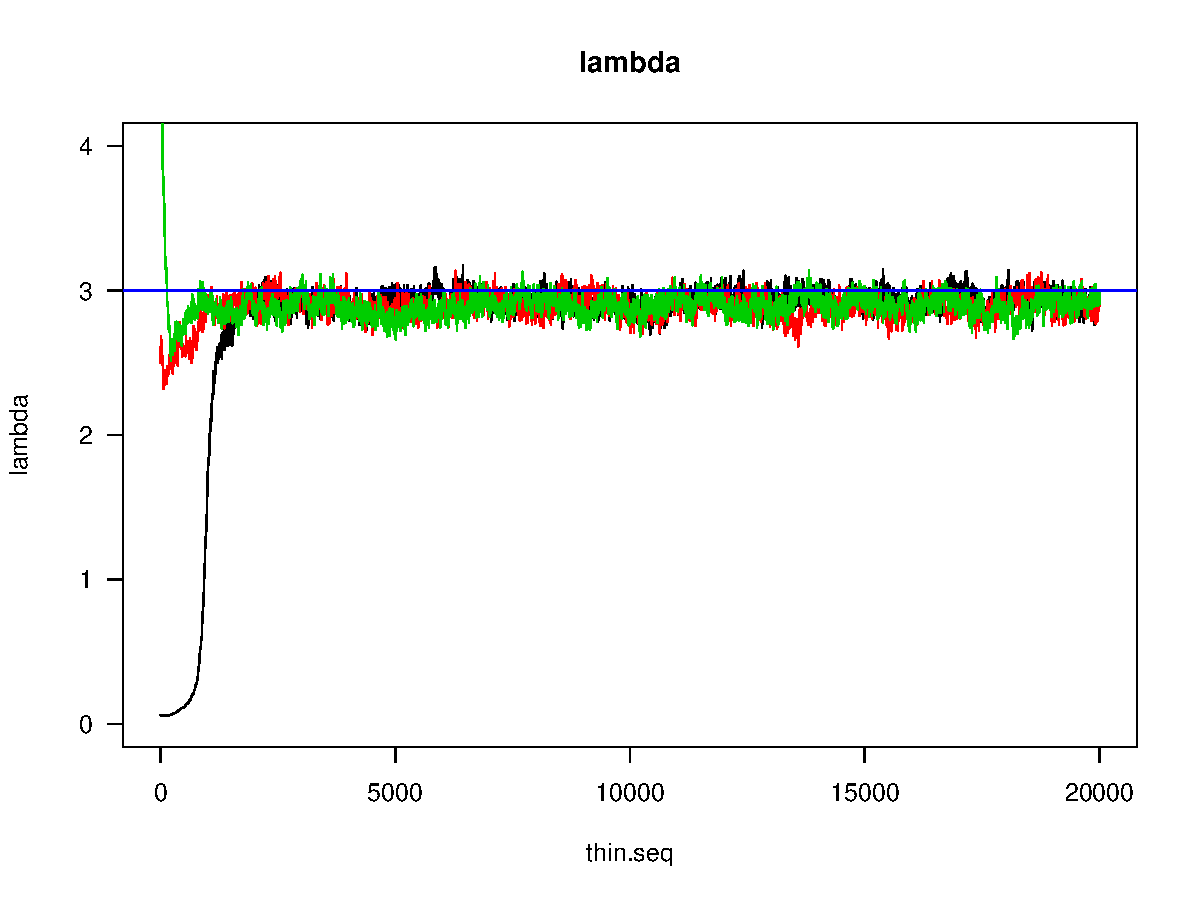
\includegraphics[width=6.0in]{fig__trace_lambda_sim.pdf}
%\label{fig_sim_sum1}
%\end{center}
%\end{figure}



%\begin{figure}[p]
%\caption{Simulation study results for $\tau^{ARC}$ where the horizontal blue lines represent the known true values of the parameters.}
%\begin{center}
%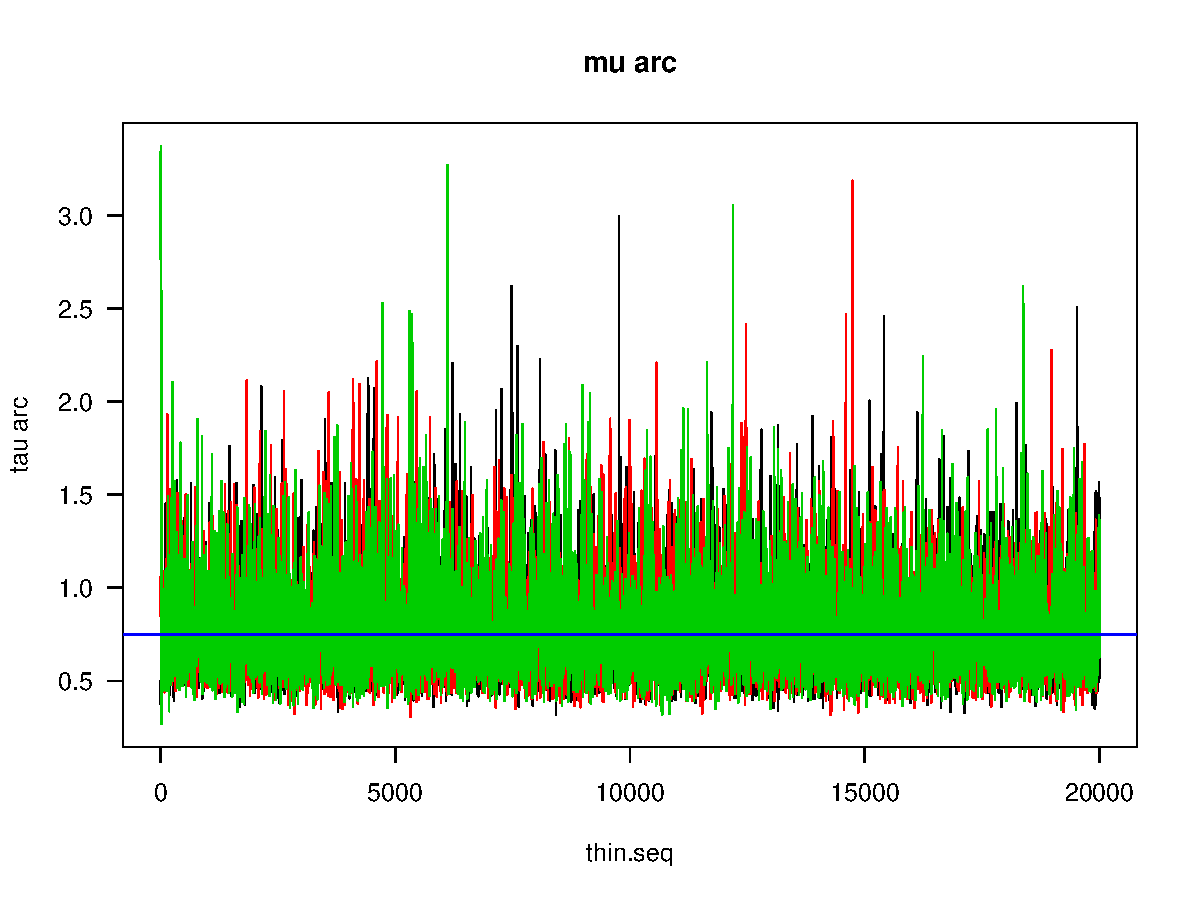
\includegraphics[scale=0.7]{test.pdf}
%\label{figure:figure1}
%\end{center}
%\end{figure}


Results for $\Sigma$ are equally as good, converging to the true parameter value before 5,000 iterations. Below we show the results for Site 1, Hagere Salaam. The remaining estimates are displayed in the Appendix. 

%\begin{figure}[htbp]
%\begin{center}
%\caption{Simulation study results for $\Sigma$ for site one (Hagere Salaam) where the horizontal blue lines represent the known true values of the parameters.}  
%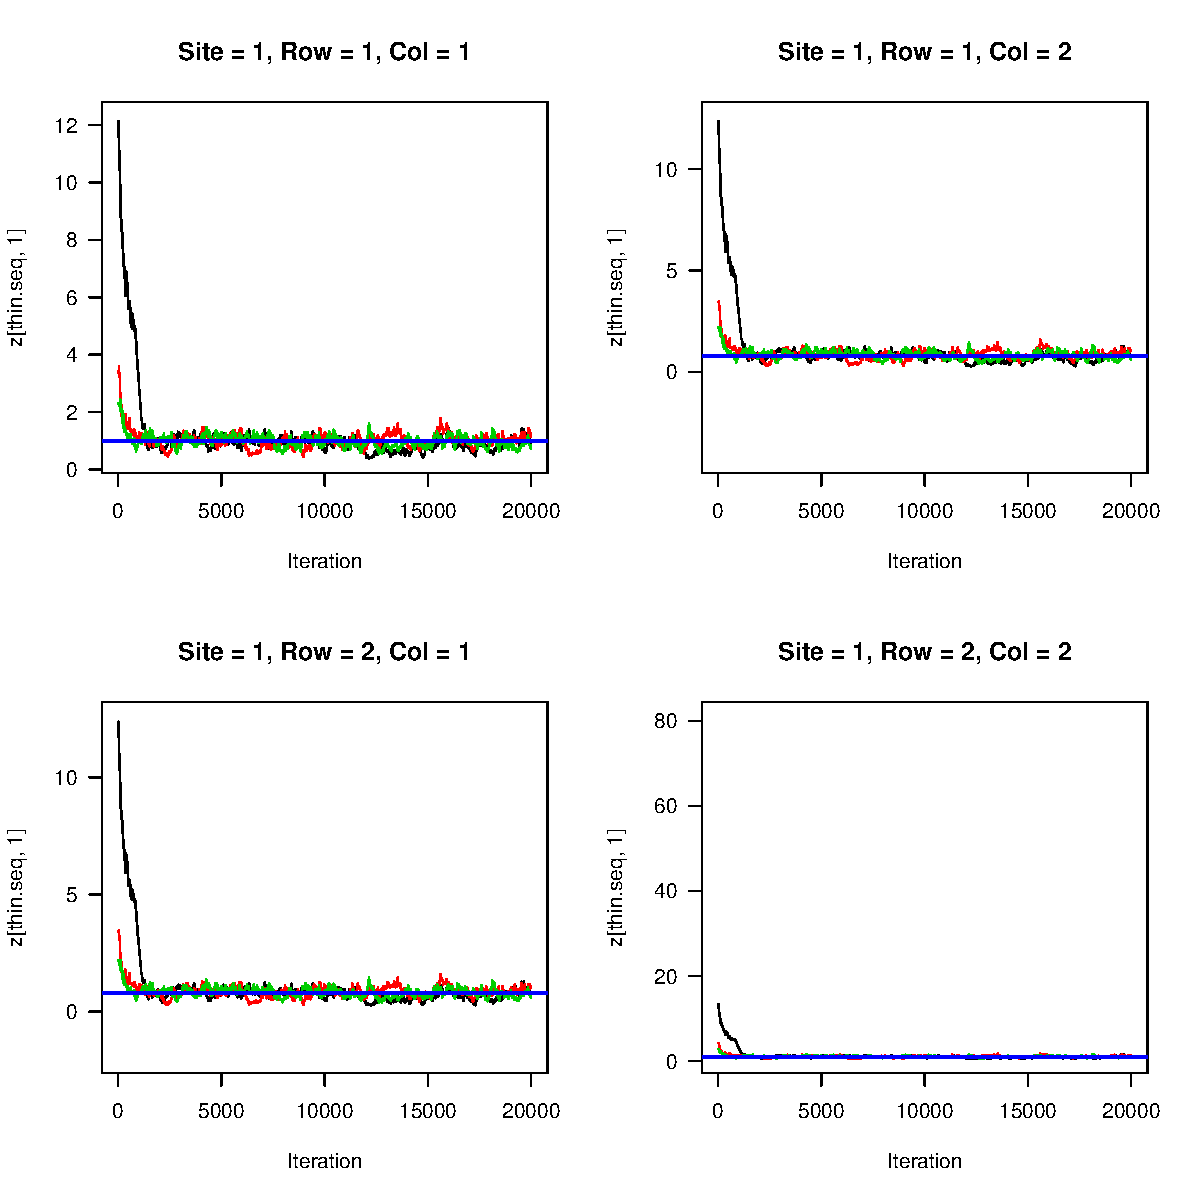
\includegraphics[page=1,width=5.0in]{fig_tobit_trace_sigma_covariance_sim.pdf}   
%\end{center}
%\end{figure}


%\begin{figure}[htbp]
%\begin{center}
%\caption{Simulation study results for $\mu^{ARC}$ where the horizontal blue lines represent the known true values of the parameters.}
%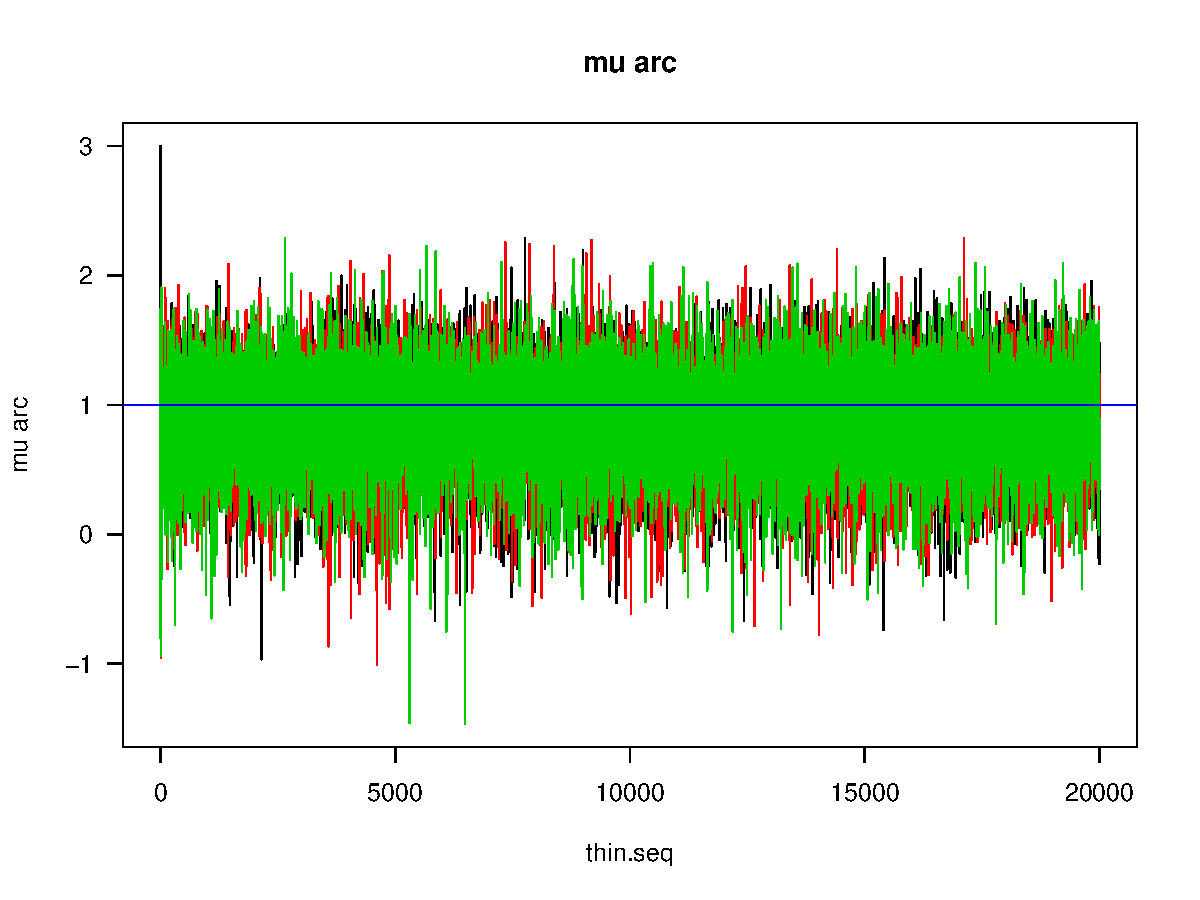
\includegraphics[width=6.0in]{fig__trace_mu.arc_sim.pdf}
%\label{fig_sim_sum1}
%\end{center}
%\end{figure}



%%%%%%%%%%%%%%%%%%%%%%%%%%%%%%%%%%%%
\section{Results}\label{sec:results}
%%%%%%%%%%%%%%%%%%%%%%%%%%%%%%%%%%%%

Our results are based on three chains of 20,000 after a burn-in of 15,000 iterations with an adaption parameter of 2,000. We assessed convergence by running the chain for three different starting values, 4 standard deviations above and below the historical means.The values of the Brooks, Gelman, and Rubin convergence diagnostic for each of the parameters, were mostly below 1.1 (lambda, tau, tau.arc, mu.arc), a threshold suggested by \cite{Gamerman1997} as satisfactory, except for the February Nino Effect ($\beta^{February}$). Results can be found in the Appendix.\footnote{We noticed that some of our samples stabilized after under 5,000 iterations, but a strong autocorrelation is present, such as with tau.}  



\subsection{Trace Plots of Key Parameters}

We ran trace plots for each parameter. Parameters for which are most interested in estimating and are typically difficult to identify $\lambda$, the distance correlation across sites, and $\Sigma$, the within site correlation matrix. 

%- We computed posterior means and standard errors for each parmater; they are available in the supplemental material
%- Plot the posterior mean of mu to show overall time series pattern
%- Related: plot the posterior mean of P(wet) and mean mm per day.


%Also include some posterior predictive checks.
 %- Mean rainfall by month
 %- Proportion of wet days per month
 %- Interannual variability



We begin by displaying $\lambda$, the parameter determining spatial correlation in our distance matrix. $\lambda$ converges to an estimate of about 0.6, while $\tau$, our parameter scaling $\lambda$ in the covariance matrix of Z, converges to 8. $\lambda$ exhibits more autocorrelation than in the simulated data. Thus for two sites $i$ and $k$ that have an euclidean distance of 1 is approximately 100 kilometers, and the $d_{ik}$ entry of the d matrix will be equal to 1, then $v_{ik}$ is $exp(-.06*1)$ is .98. In general our spatial correlations for the V matrix range from .95 to .99. 

Tau is estimated at 8.8 mm.

The mean of beta arc (mu.arc) is approximately 0.7 with a  variance of 2.2? (tau.arc), so the ARC satellite has a slightly positive bias on rainfall above and beyond a rain gauge. 


%\begin{figure}[htbp]
%\caption{Trace of $\lambda$, Scalar on Distance Matrix for V}
%\begin{center}
%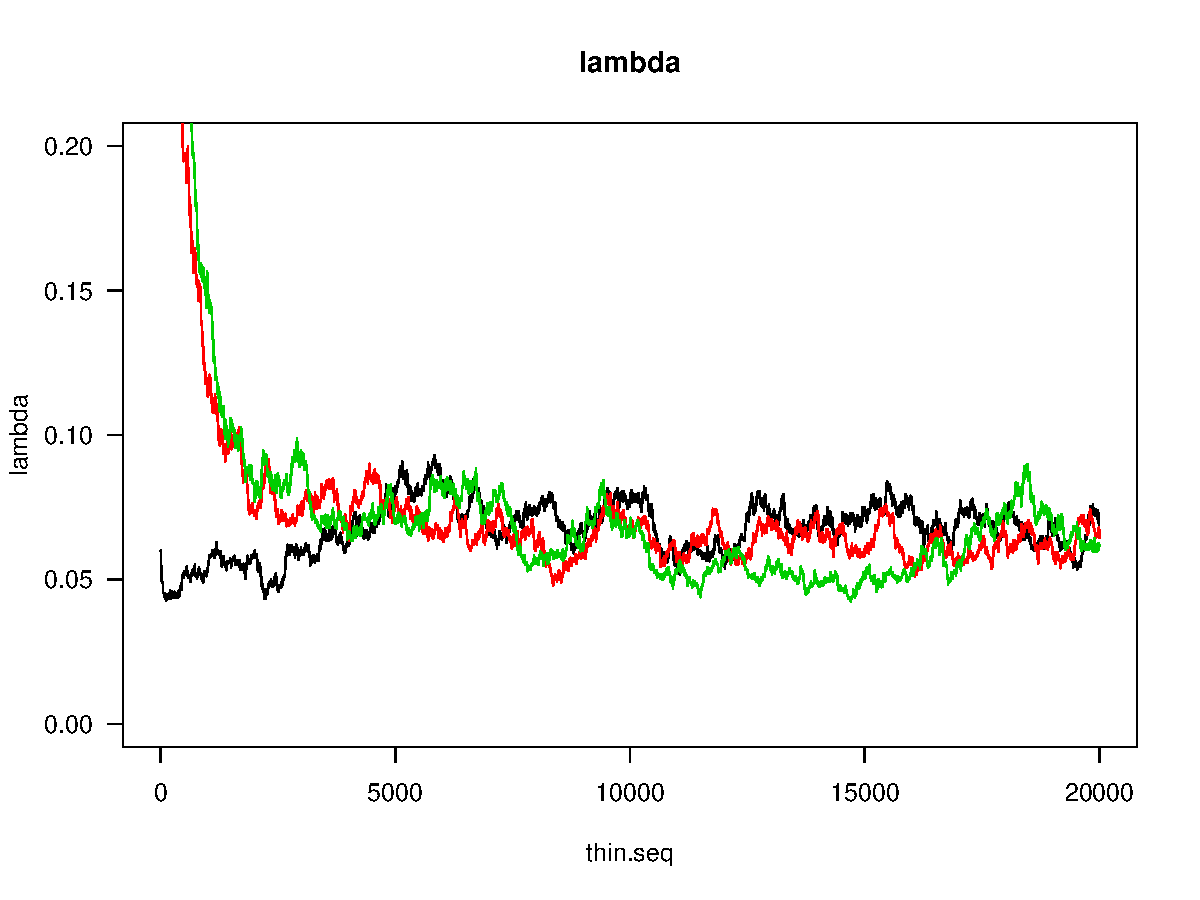
\includegraphics[width=5.0in]{fig__trace_lambda.pdf}
%\end{center}
%\end{figure}



%\begin{figure}[htbp]
%\caption{Trace of $\tau$, Scalar on Covariance Matrix of Z}
%\begin{center}
%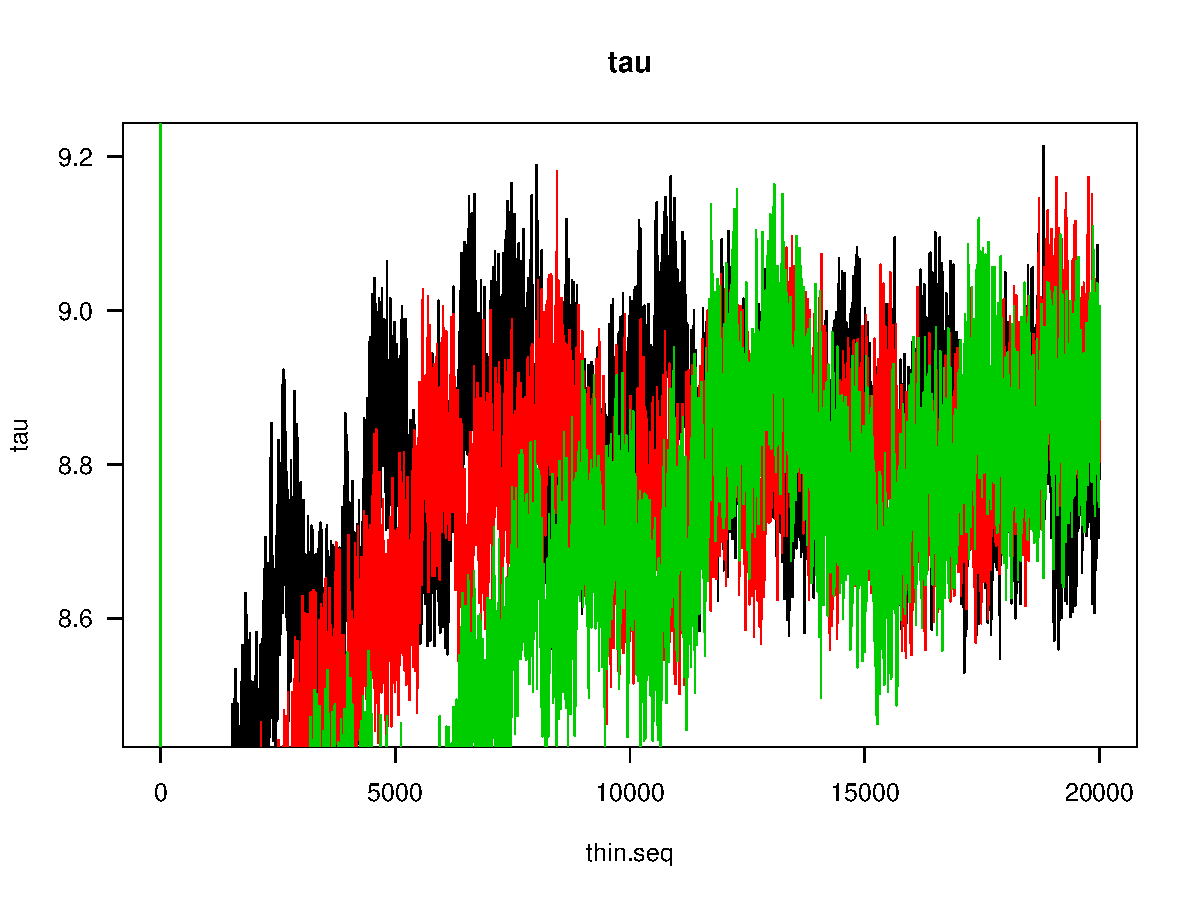
\includegraphics[width=5.0in]{fig__trace_tau.pdf}
%\end{center}
%\end{figure}




%\begin{figure}[htbp]
%\caption{Trace of $\beta^{Arc}$, Bias of Using Arc Satellite Measure}
%\begin{center}
%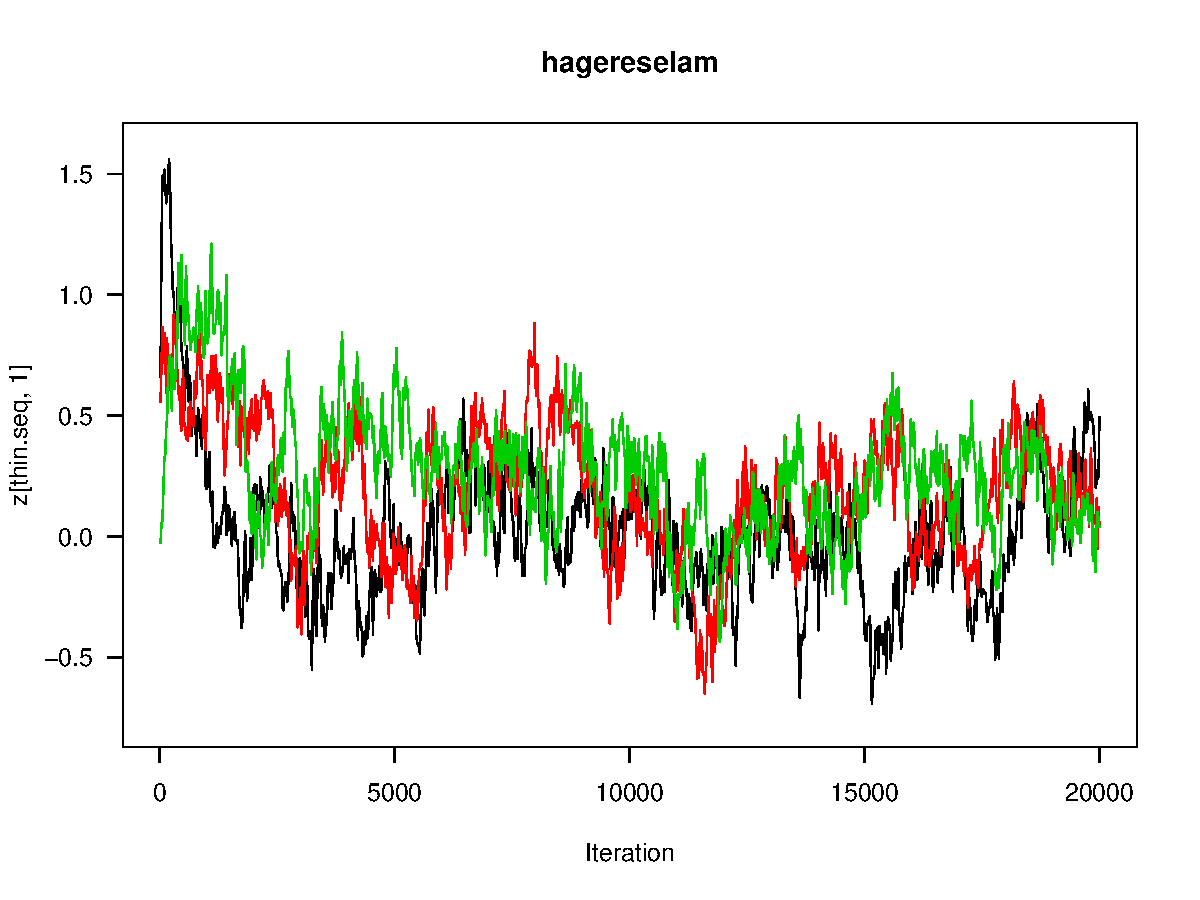
\includegraphics[width=5.0in]{fig_tobit_trace_beta_arc.pdf}
%\end{center}
%\end{figure}

%\begin{figure}[htbp]
%\caption{Trace of $\beta$'s}
%\begin{center}
%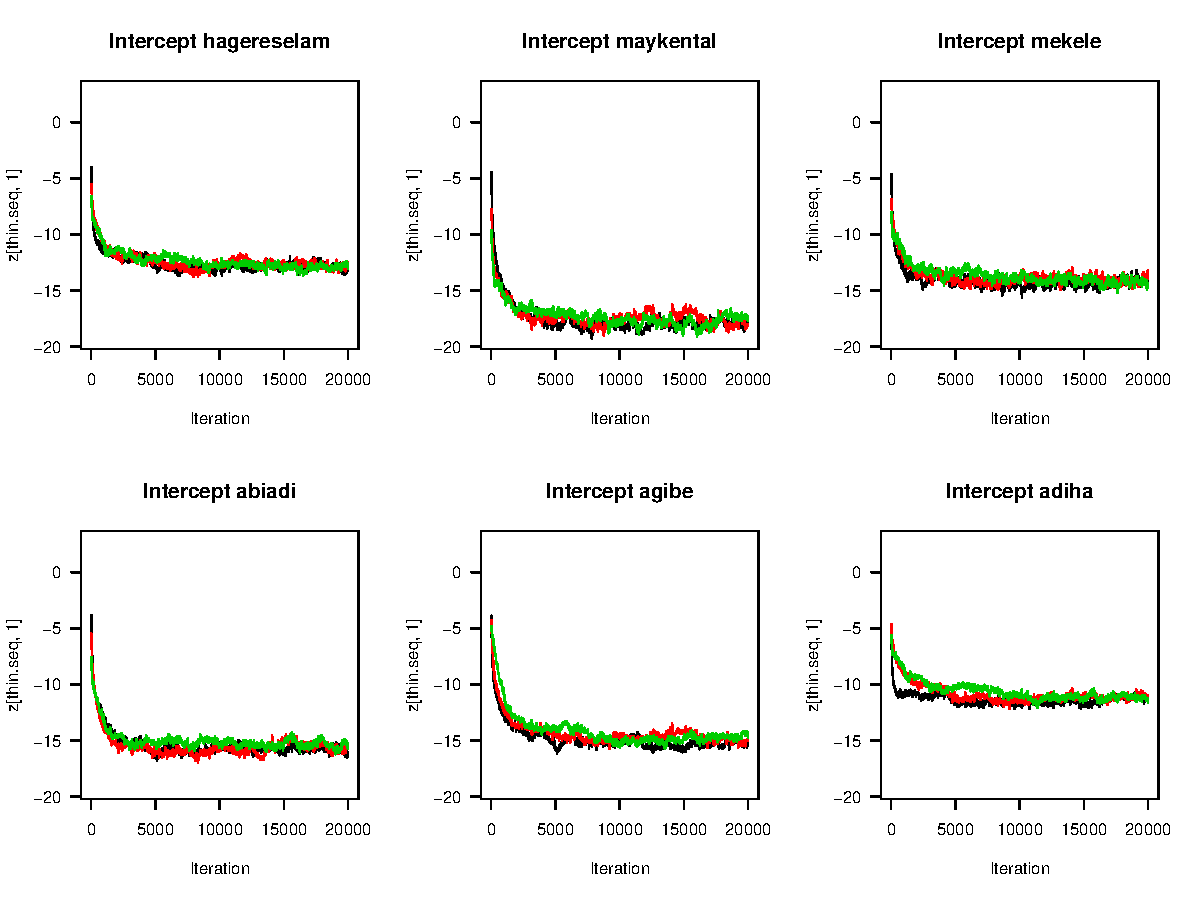
\includegraphics[width=5.0in]{fig_tobit_trace_beta_P23.pdf}
%\end{center}
%\end{figure}

%\begin{figure}[htbp]
%\caption{Trace of $\beta$s' Mean, Mu}
%\begin{center}
%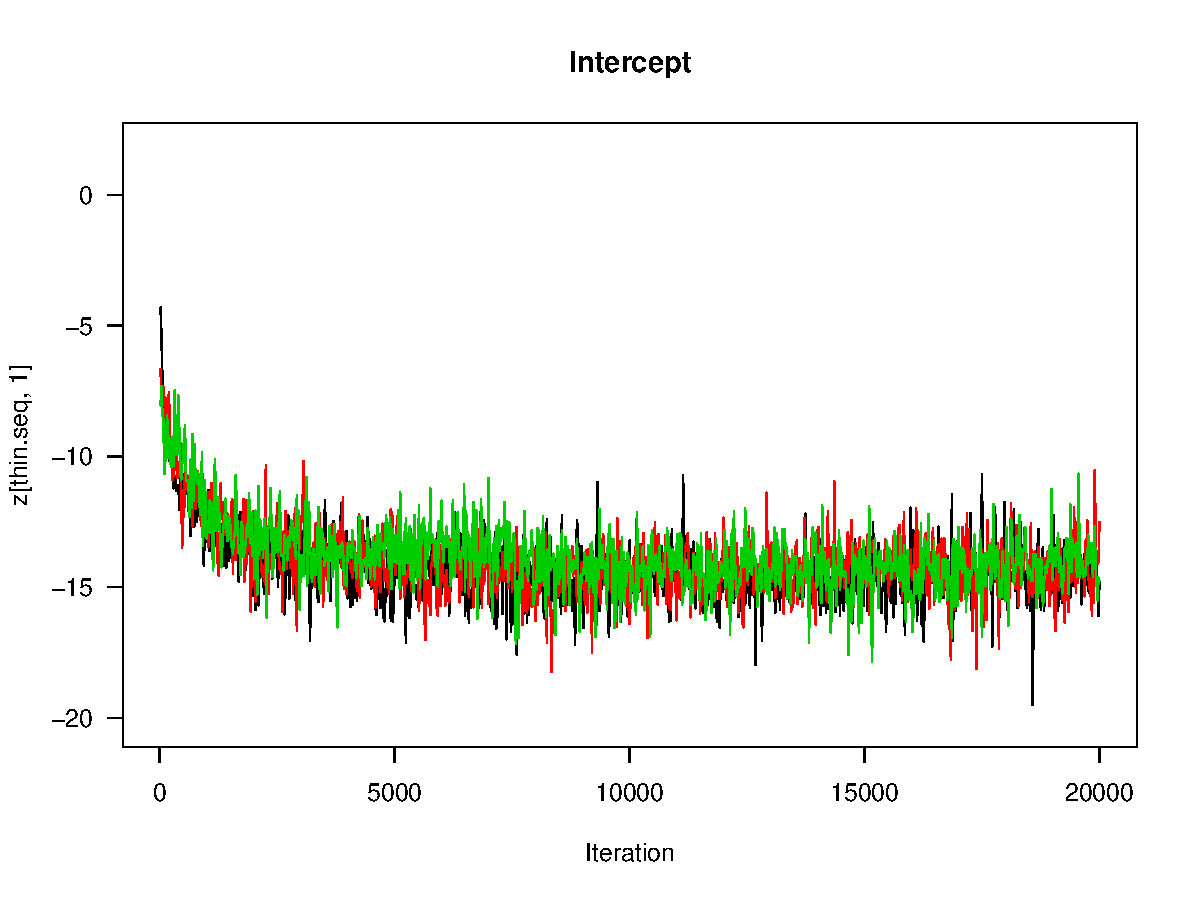
\includegraphics[width=5.0in]{fig_tobit_trace_mu.pdf}
%\end{center}
%\end{figure}


%\begin{figure}[htbp]
%\caption{Trace of $\Sigma$, Location Specific Covariances (Hagere Salaam) }
%\begin{center}
%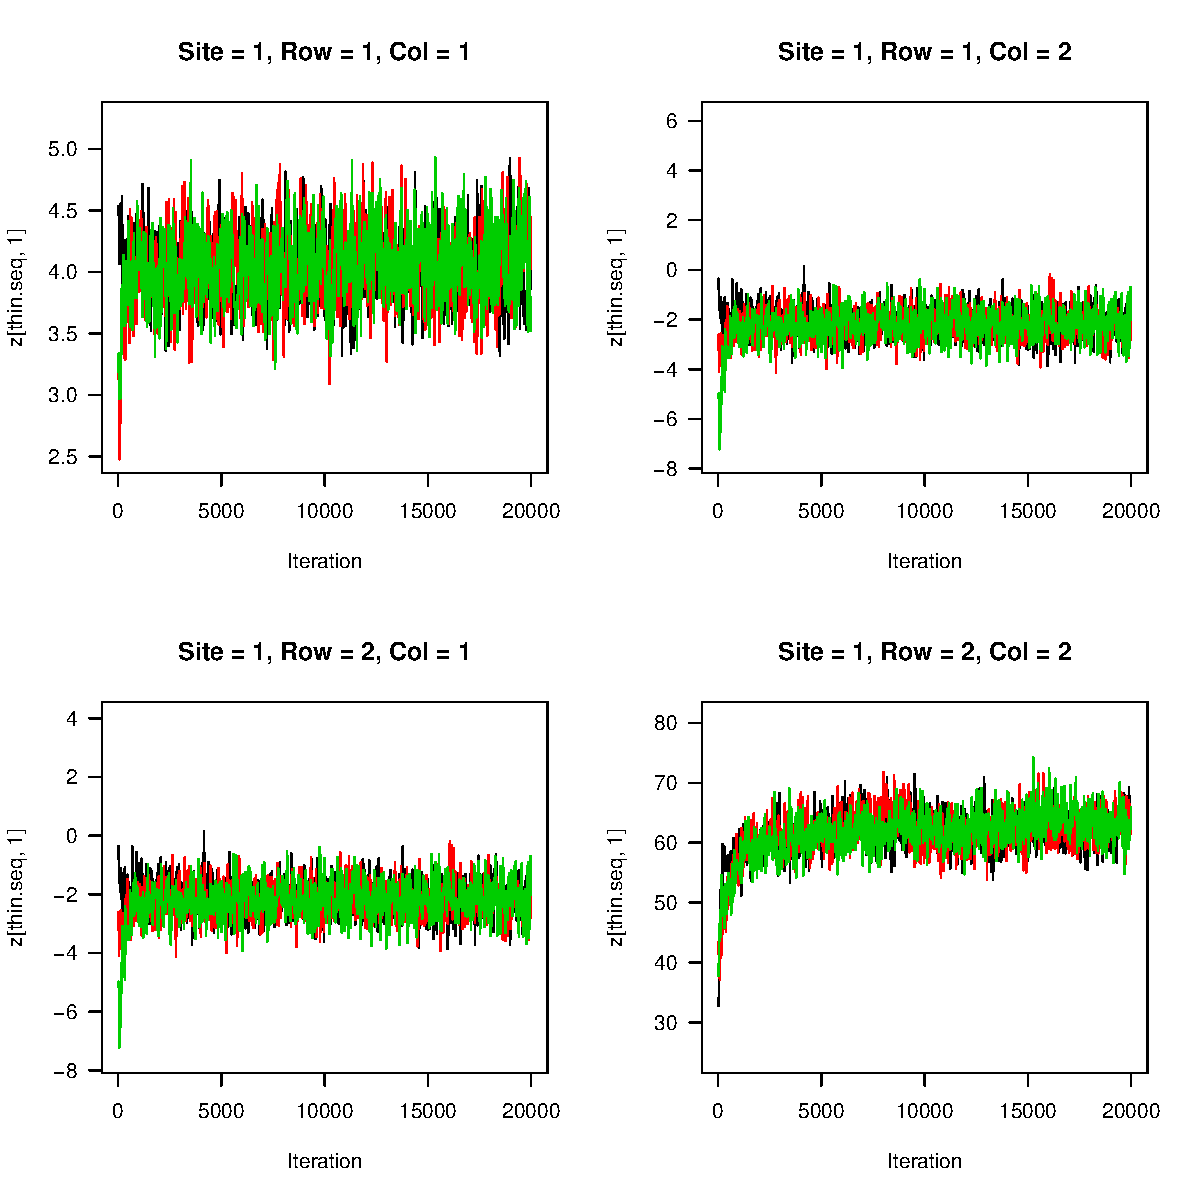
\includegraphics[page=1,width=5.0in]{fig_tobit_trace_sigma_covariance.pdf}     
%\end{center}
%\end{figure}

%\begin{figure}[htbp]
%\caption{Trace of $\sigma$, variance of betas}
%\begin{center}
%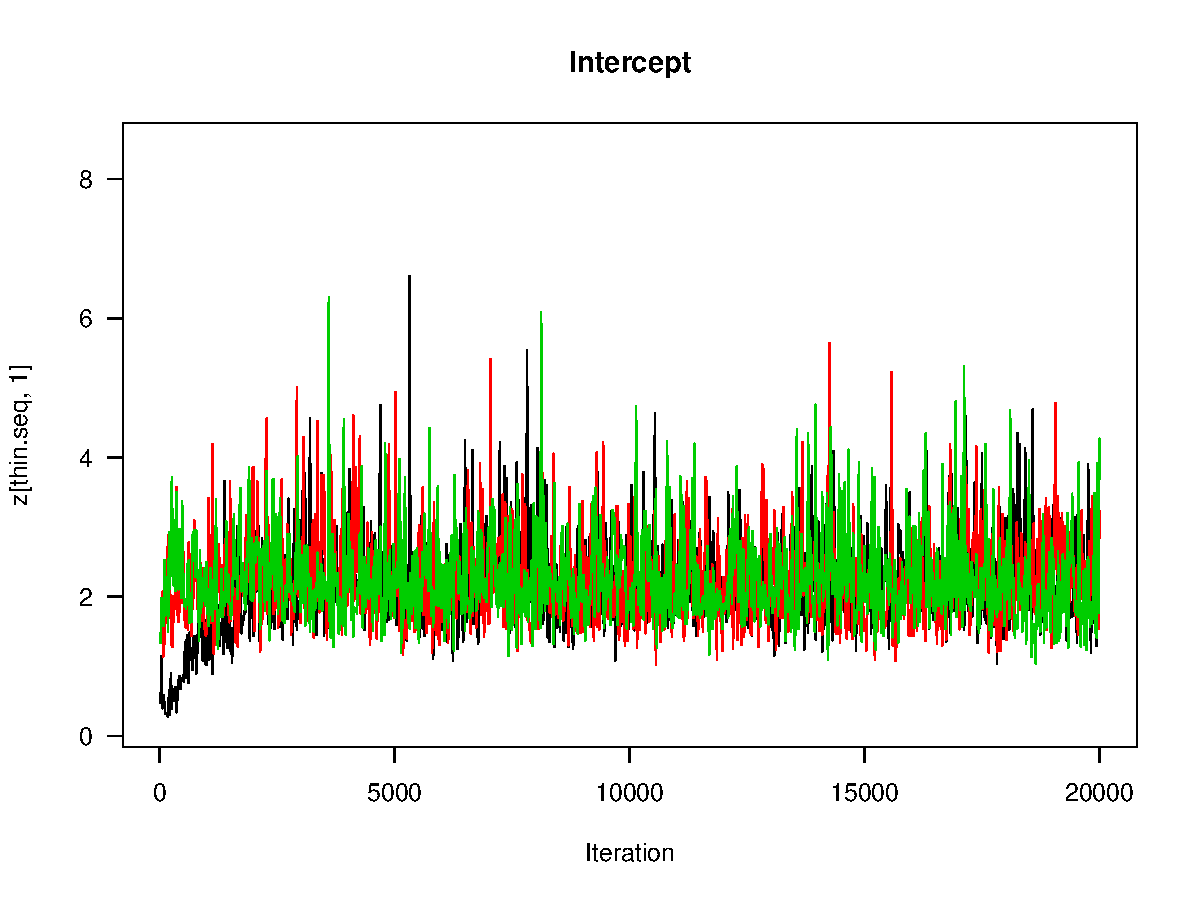
\includegraphics[width=5.0in]{fig_tobit_trace_sigma.pdf}
%\end{center}
%\end{figure}



%\includegraphics[width=6.0in]{Posterior_pwet_series8.pdf}
%\includegraphics[width=6.0in]{Posterior_pwet_series9.pdf}
%\caption{Simulation study results for $\lambda$, $\mu_\alpha$, and $\tau_\alpha$, where the horizontal blue lines represent the known true values of the parameters.}
%\label{Posterior}

\section{Rainfall Metrics Measured}
\label{sec:metrics}

We have shown that our model performs well in terms of recovering parameters using simulated data, and it converges relatively quickly to its posterior estimates using real rainfall data. An additional motivation of this paper is to be able to predict higher level metrics such as: onset of rainfall within a season, inter-annual rainfall variability, and the number of consecutive dry days per year. In developing countries, where smallholder farmers have little savings and or capital to shield their risk, accuracy in predicting these measures can be the difference between a successful and devastating harvest. For example, yields can be heavily affected by planting a week too early or too late with respect to rainfall onset. Knowing consecutive dry days helps in preparing for a dry season, and inter-annual variability gives us a sense of the upper and lower bounds for rainfall over time. 

We begin by plotting first some basic posterior estimates for mean rainfall and the proportion of wet days per month. We then follow with some of the harder to predict diagnostics: inter-annual rainfall variability, probability of consecutive dry days, probability of rainfall onset.



%\begin{figure}[htbp]
%\caption{Posterior Mean Rainfall }
%\begin{center}
%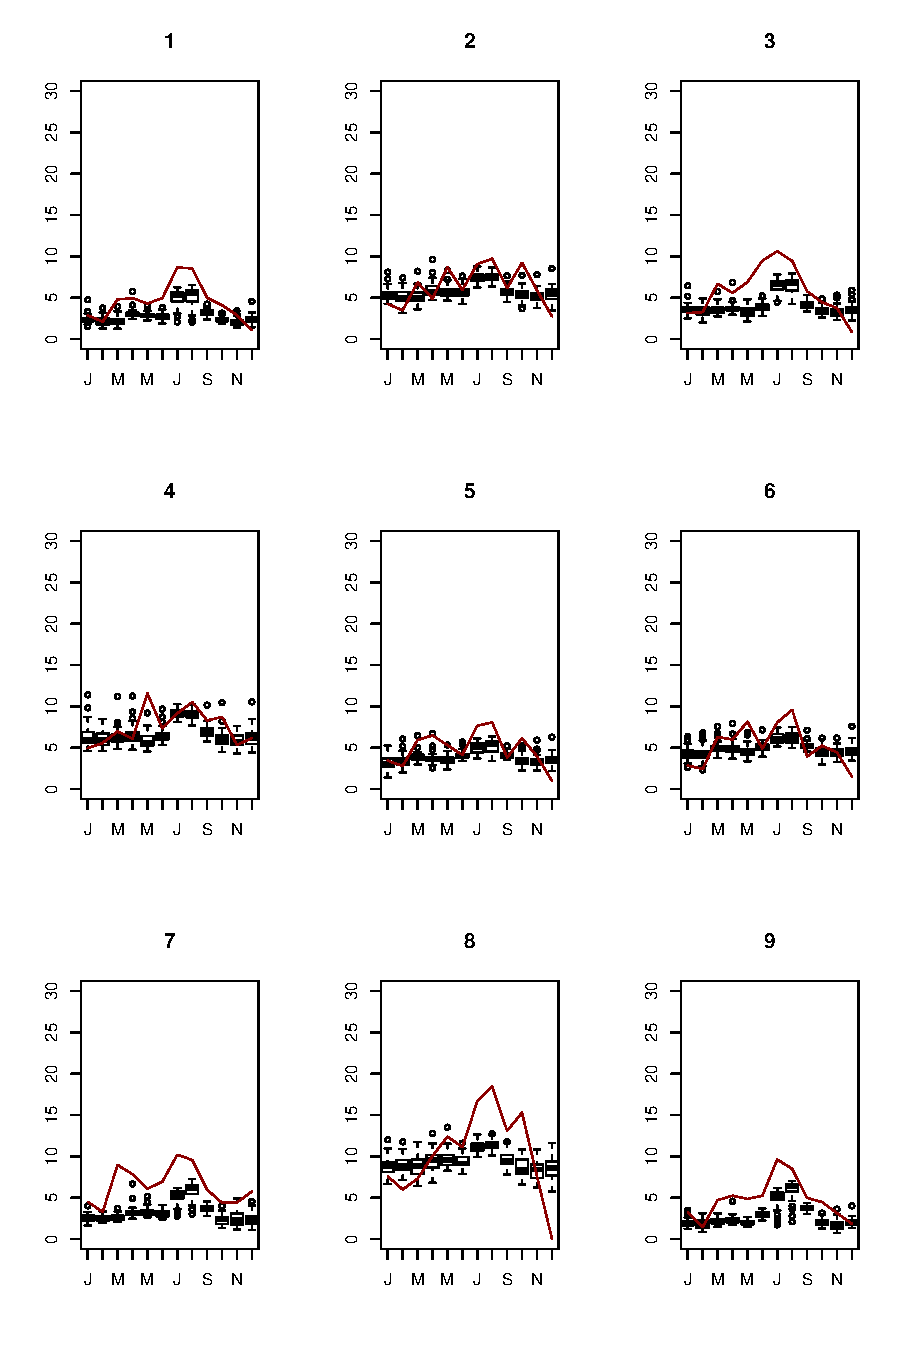
\includegraphics[width=5.0in]{Posterior_mean_series.pdf}
%\end{center}
%\end{figure}

%\begin{figure}[htbp]
%\caption{Posterior Probability of Rainfall}
%\begin{center}
%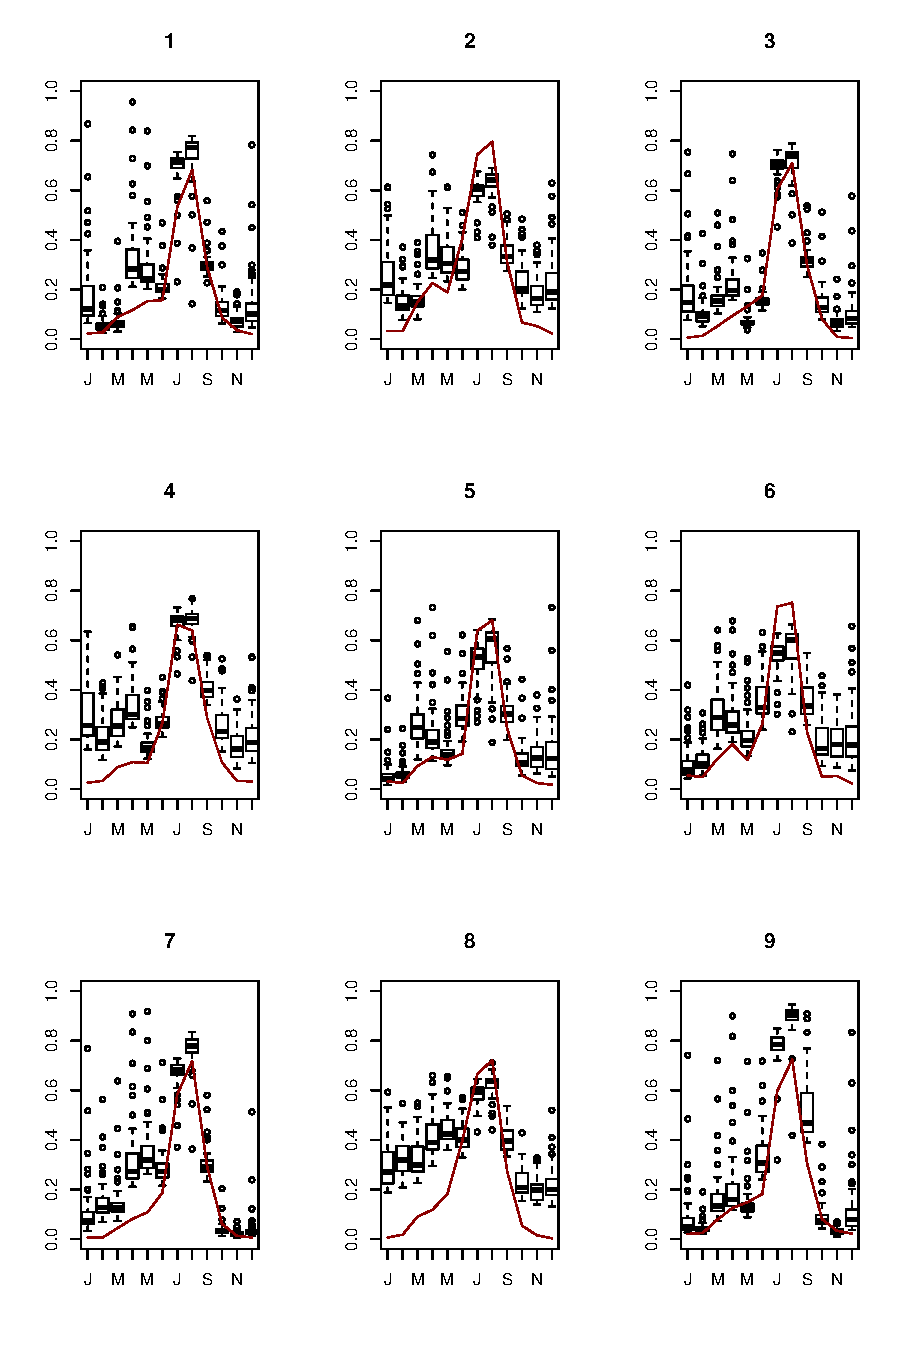
\includegraphics[width=5.0in]{Posterior_pwet_series.pdf}
%\end{center}
%\end{figure}


%\begin{figure}[htbp]
%\caption{Rainfall Onset using Simulated Rainfall}
%\begin{center}
%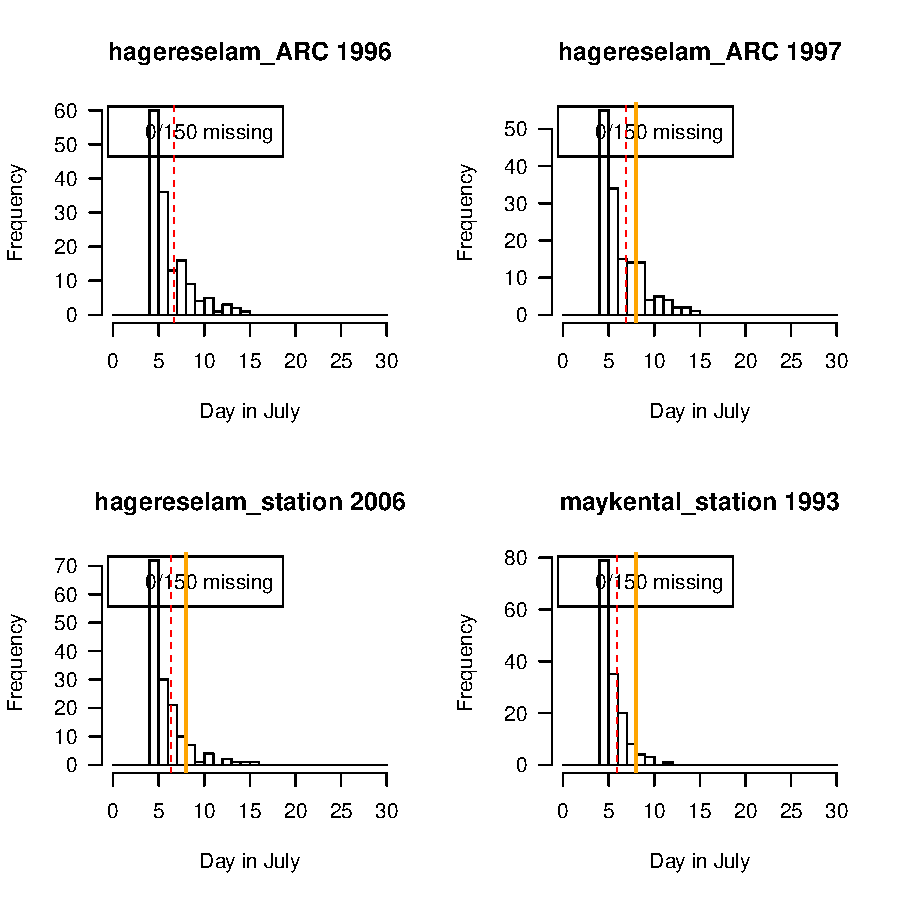
\includegraphics[width=5.0in]{Onset_postpred.pdf}
%\end{center}
%\end{figure}


%\begin{figure}[htbp]
%\caption{Inter-annual Rainfall Variability using Simulated Rainfall}
%\begin{center}
%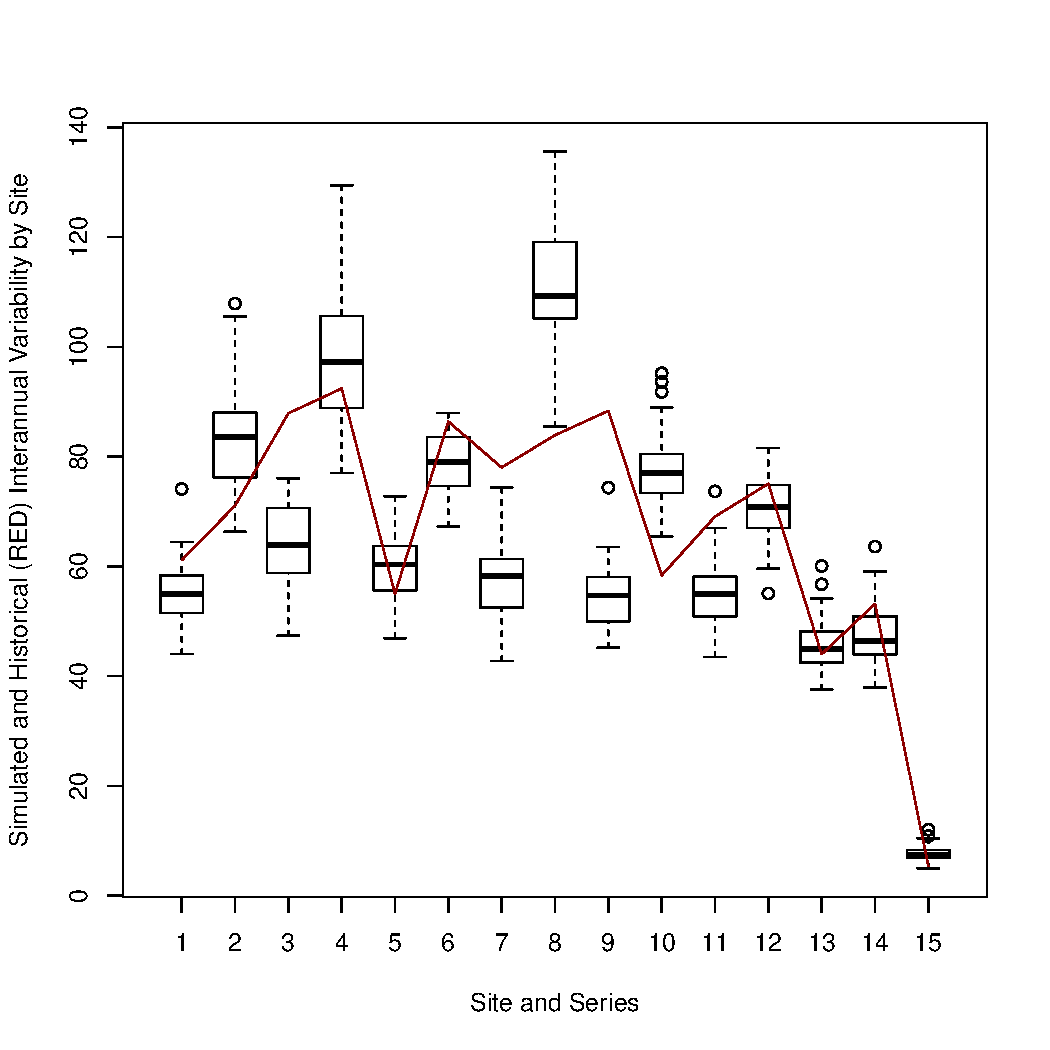
\includegraphics[width=5.0in]{Interannual.pdf}
%\end{center}
%\end{figure}

%\begin{figure}[htbp]
%\caption{Number of Consecutive Dry Days ($>$3 days} using Simulated Rainfall}
%\begin{center}
%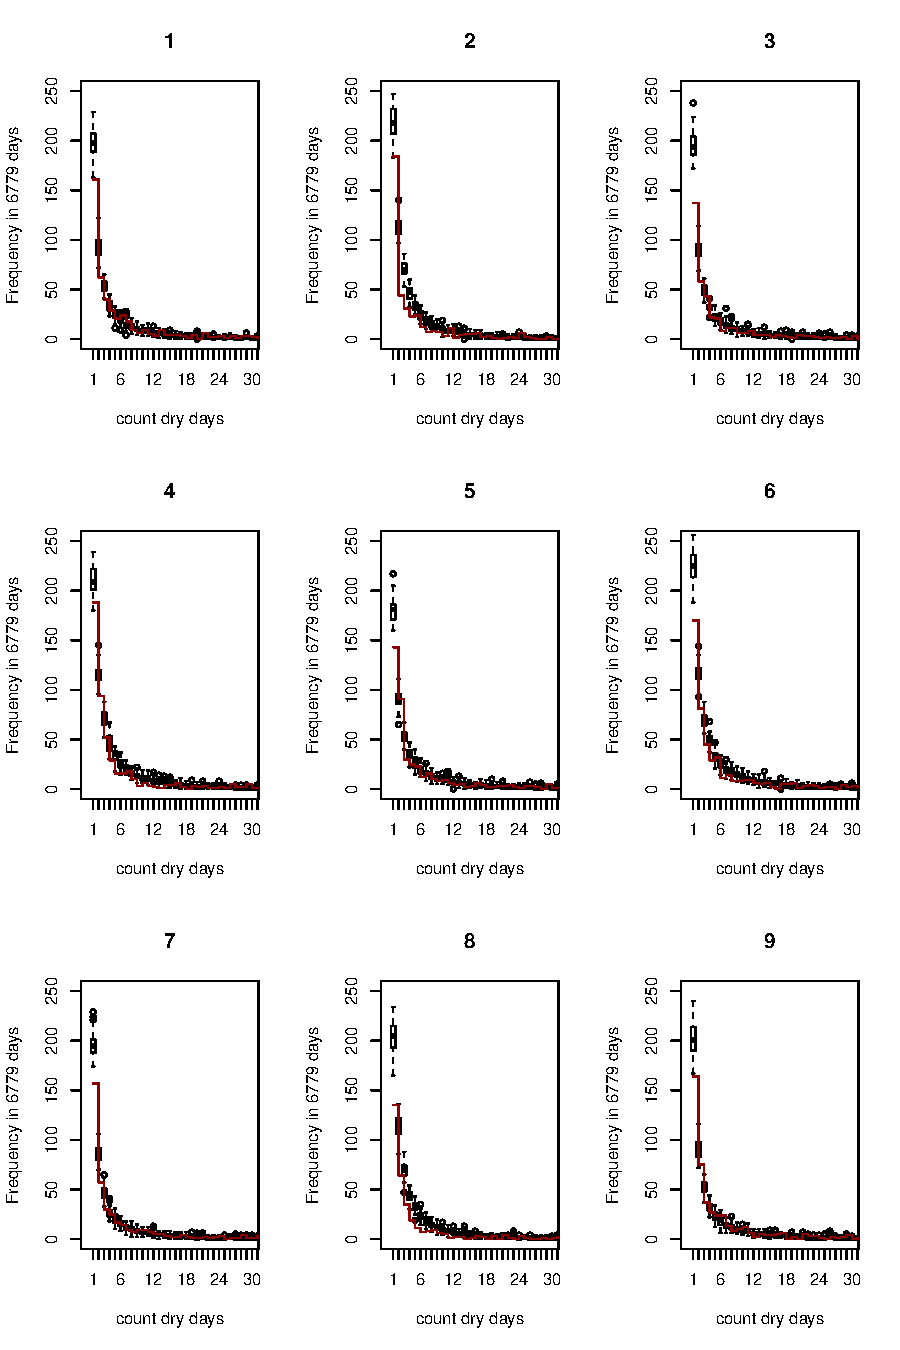
\includegraphics[width=5.0in]{Consec_Data_Series.pdf}
%\end{center}
%\end{figure}


%%%%%%%%%%%%%%%%%%%%%%%%%%%%%%%%%%%%%%%%%%
\section{Discussion}\label{sec:discussion}
%%%%%%%%%%%%%%%%%%%%%%%%%%%%%%%%%%%%%%%%%%

We have considered a model where rainfall is a latent multivariate t-distribution, driven by seasonal patterns, satellite measurement error, and within site correlation between time series. The model is fitted using Monte Carlo methods with Gibbs and Metropolis Hastings sampling. Initial starting values in the three chains are set at the historical means, and then four standard deviations above and below the means. The model's accuracy is tested on simulated data and performs well, recovering all of our predetermined parameters. The hierarchical structure allows for fitting within site correlations of various time series measured at a single location, as well across site spatial correlations. Both features enable us to incorporate information on rainfall patterns that can improve out of sample simulations of rainfall, as well as tougher to estimate rainfall characteristics: inter-annual rainfall variability, probability of consecutive dry days, probability of rainfall onset.

The ability to incorporate spatial, temporal, and measurement correlations has important policy implications. First, food insecurity is generally correlated over time and space in parallel with rainfall patterns. Thus, predictions that incorporate these spatial patterns can allow for better response to anticipated droughts and subsequent food shortages in a region. This is crucial for aid organizations and first responders to such crises. Second, different satellite measurements can detect and depict different weather patterns depending on their resolution and what they aim to measure: cloud cover, vegetation, lights, etc. Incorporating multiple information sets around a particular area can increase the accuracy with which we predict weather patterns by narrowing the variance around the mean trends. Although this research does not present a new weather generator for use by end-users, we hope that the methodological advances made will eventually lead to such a tool. 




%%%%%%%%%%%%%%%%%%%%%%%%%%%%%%%%%%%%%
\newpage
\section{Appendix}\label{sec:appendix}
%%%%%%%%%%%%%%%%%%%%%%%%%%%%%%%%%%%%%

The full posterior can be written as
\begin{align*}
p(\btheta \mid \bY) \propto \prod_{s = 1}^S \prod_{t = 1}^T \prod_{j = 1}^{J_s} & p(Y_{stj} \mid W_{stj}) p(W_{stj} \mid Z_{st}, \beta_s^\text{ARC}, \Sigma_s, \gamma_{st}) p(Z_{st} \mid \bbeta_s^Z, \tau, \lambda) \\
& p(\bbeta_s^Z | \bmu, \bsigma) p(\beta_s^\text{ARC} \mid \mu^\text{ARC}, \tau^\text{ARC}) \\
& p(\bmu) p(\bsigma) p(\tau) p(\lambda) p(\mu^\text{ARC}) p(\tau^\text{ARC}) p(\bSigma_s) p(\gamma_{st}),
\end{align*}
where $\btheta$ denotes the entire vector of parameters, 
$$
\btheta = \{\bW, \bZ, \bbeta^\text{ARC}, \bSigma, \bgamma, \bbeta^Z, \tau, \lambda, \bmu, \bsigma, \mu^\text{ARC}, \tau^\text{ARC}\}.
$$

To sample from this posterior, we use MCMC. First we set initial values of $\lambda$, $\tau$, $\mu^\text{ARC}$, $\tau^\text{ARC}$, $\mu_p$ and $\sigma_p$ (for $p = 1, ..., 23$), $\bSigma_s$ (for $s = 1, ..., S$), and $\gamma_{st}$ (for $s = 1, ..., S$ and $p = 1, ..., P$). These initial values are set to be overdispersed around rough estimates of the parameters based on fits of smaller, simpler models to the data. Next we sample initial values of
\begin{align}
\beta_s^\text{ARC} &\mid \mu^\text{ARC}, \tau^\text{ARC}\text{ (for }s = 1, ..., S), \\
\beta^Z_{sp} &\mid \mu_p, \sigma_p\text{ (for }s = 1, ..., 6\text{ and }p = 1, ..., P), \\
\bZ_t &\mid \bbeta^Z, \lambda, \tau, \bX_t\text{ (for }t = 1, ..., N).
\end{align}

Then, for iteration $g = 1, 2, ...., G$, where we set $G = 5000$, we perform the following steps:
\begin{enumerate}

% W
\item Sample $\bW \mid \bY, \bgamma, \bZ, \bbeta^\text{ARC}, \bSigma$.\\
The conditional posterior distribution of the length-$J_s$ latent rainfall vector for location $s$ and day $t$, $\bW_{st}$, follows the multivariate normal distribution described in Equation 2 from Section 3. Each element of this vector can be sampled, conditional on the other elements, from a univariate normal distribution according to standard methods (cite). This draw is made in one of three ways:
\begin{enumerate}
\item Case 1: If $Y_{stj} > 0$, then $W_{stj} = Y_{stj}$; in other words, no sample is drawn, but instead the value of $W_{stj}$ is fixed.
\item Case 2: If $Y_{stj} = 0$, then the univariate normal distribution from which $W_{stj}$ is sampled  is truncated on the right by zero, since the model specifies that the latent rainfall amount must be less than zero in this case.
\item Case 3: If $Y_{stj}$ is missing, then the sample is drawn without any truncation, since the missing observation, $Y_{stj}$, could have been equal to zero or greater than zero.
\end{enumerate}

% gamma
\item Sample $\bgamma \mid \bW, \bZ, \bbeta^\text{ARC}, \bSigma, \alpha$. \\
$
\gamma_{st} \sim \Gamma(\text{shape = }(J_s + \alpha)/2, \text{ rate = }2/((\bW_{st} - \bmu^W_{st})^T\Sigma_s^{-1}(\bW_{st} - \bmu^W_{st}) + \alpha)),\\
$ where
$
\bmu^W_{st} = \mathbf{1}Z_{st} + \bX_{s}^\text{ARC}\beta_s^\text{ARC},
$
for $s = (1, ..., S)$ and $t = (1, ..., N)$, and $\alpha$ is set to 5.

% Z
\item Sample $\bZ \mid \bW, \bgamma, \bbeta^\text{ARC}, \bSigma, \bbeta^Z, \tau, \lambda$. \\
The spatial mean rainfall vector can be sampled in closed form from a multivariate normal distribution. To compute the mean and variance of its multivariate normal posterior distribution, we ``complete the square" twice. First, note that the posterior distribution of $\bZ_t$ is proportional to
$$
p(\bW \mid \bY, \bgamma, \bZ, \bbeta^\text{ARC}, \bSigma) p(\bZ \mid \bbeta^Z, \tau, \lambda),
$$
where both of these terms are multivariate normal probability distribution functions (PDFs). In the first term, by treating $\bZ$ as unknown and the other parameters as known, one can see that it is proportional to the multivariate normal PDF where
$$
\bZ_t \sim \text{N}_S(\bmu^Z_t, \bSigma_t^Z),
$$
where the $s^\text{th}$ element of the mean is given by
$$
\mu^Z_{st} = (\mathbf{1})^T \Sigma_s^{-1}(\bW_{st} - \bX_s^\text{ARC}\beta_s^\text{ARC})/(\mathbf{1}^T \Sigma_s^{-1} \mathbf{1}),
$$
the variance of the $s^\text{th}$ element is given by
$$
\Sigma_{t[s]}^Z = 1/(\gamma_{st}\mathbf{1}^T \Sigma_s^{-1} \mathbf{1}),
$$
and the off-diagonal elements of $\Sigma_t^Z = 0$.

Next, combining this term with the second term, which is also a multivariate normal PDF, we compute the full conditional posterior distribution for $\bZ_t$:
$$
\bZ_t \sim \text{N}_S\Biggl(\Bigl((\bSigma_t^Z)^{-1} + (\sigma^2\bV)^{-1}\Bigr)^{-1}\Bigl((\bSigma_t^Z)^{-1}\bmu_t^Z + (\sigma^2\bV)^{-1}\bX_t\bbeta^Z\Bigr), \Bigl((\bSigma_t^Z)^{-1} + (\sigma^2\bV)^{-1}\Bigr)^{-1}\Biggr).
$$

% Beta-ARC
\item Sample $\bbeta^\text{ARC} \mid \bW, \bgamma, \bZ, \bSigma, \mu^\text{ARC}, \tau^\text{ARC}$ from
$$
\beta_s^\text{ARC} \sim \text{N}\Biggl(\frac{\mu_s^W/\sigma_s^2(W) + \mu^\text{ARC}/\tau_\text{ARC}^2}{1/\sigma_s^2(W) + 1/\tau_\text{ARC}^2}, \frac{1}{1/\sigma_s^2(W) + 1/\tau_\text{ARC}^2}\Biggr),
$$
where
$$
\mu_s^W = \frac{-(\bX_s^\text{ARC})^T \bSigma_s^{-1} \sum_{t = 1}^N \gamma_{st} (\mathbf{1} Z_{st} - \bW_{st})}{\sum_{t=1}^T \gamma_{st}(\bX^{ARC}_s)^T \Sigma_s^{-1} \bX_s^\text{ARC}}
$$
and
$$
\sigma_s^2(W) = 1/\sum_{t=1}^N \gamma_{st}(\bX^\text{ARC}_s)^T \Sigma_s^{-1} \bX_s^\text{ARC}.
$$

% Sigma
\item Sample $\bSigma \mid \bW, \bgamma, \bZ, \bbeta^\text{ARC}$ from \\
$$
\Sigma_s \sim \text{Inv-Wishart}\Bigl(\text{df = }N + J_s, \text{ , scale = diag}(J_s) + \sum_{t=1}^N \gamma_{st}(\bW_{st} - \bmu^W_{st})(\bW_{st} - \bmu^W_{st})^T\Bigr),
$$
where 
$
\bmu^W_{st} = \mathbf{1}Z_{st} + \bX_{s}^\text{ARC}\beta_s^\text{ARC}.
$

% beta^Z
\item Sample $\bbeta^Z \mid \bZ, \lambda, \tau, \bmu, \bsigma$. \\
$\bbeta^Z$ is expressed as a 23 $\times S$ matrix, but its posterior distribution will be drawn from a $23 \times S = 138$-dimensional multivariate normal distribution. The variance, $\bB$, can be expressed as:
$$
\bB = \Biggl(\Bigl(\tau^2\bV \otimes (\bX^T\bX)^{-1}\Bigr)^{-1} + \Bigl(\text{Diag}(S) \otimes \text{Diag}(\bsigma)\Bigr)^{-1}\Biggr)^{-1},
$$
where $\otimes$ is the Kronecker product. The conditional posterior mean of $\bbeta^Z$ can be expressed as:
$$
\hat{\bbeta}^Z = \bB\Bigl(\text{vec}(\bX^T\bZ(\tau^2\bV)^{-1}) + (\text{Diag}(S) + \text{Diag}(\bsigma))^{-1} \text{vec}(\bmu\mathbf{1})\Bigr),
$$
where $\text{vec}(\bA)$ indicates the stacked columns of the matrix $\bA$, and $\mathbf{1}$ denotes the 1 $\times$ 6 matrix of ones, in this case.

% sigma_p
\item Sample $\bsigma \mid \bbeta^Z, \bmu$. \\
We draw $\sigma_p$ using a random-walk Metropolis step for $p = 1, ..., P$.

% mu_p
\item Sample $\bmu \mid \bbeta^Z, \bsigma$. \\
$$
\mu_p \sim \text{N}\Bigl(\sigma_0^2\bar{\beta}^Z_p/(\sigma_p^2/S + \sigma_0^2), (1/\sigma_0^2 + S/\sigma_p^2)^{-1}\Bigr),
$$
where $\sigma_0 = 5$ as in equation [].

% lambda
\item Sample $\lambda \mid \bZ, \bbeta^Z, \tau$. \\
We draw $\lambda$ using a random-walk Metropolis step.

% tau
\item Sample $\tau \mid \bZ, \bbeta^Z, \lambda$, from
$$
\tau \sim \text{Inv-Gamma}(a = 1 + NS/2, 1 + 1/2 \sum_{t=1}^N (\bZ_t - \bX_t\bbeta^Z)^T \bV^{-1} (\bZ_t - \bX_t \bbeta^Z).
$$

% mu^ARC
\item Sample $\mu^\text{ARC} \mid \beta^\text{ARC}, \tau^\text{ARC}$, from
$$
\mu^\text{ARC} \sim \text{N}\Biggl(\frac{S\bar{\beta}^\text{ARC}/\tau_\text{ARC}^2}{1 + S/\tau_\text{ARC}^2}, \sqrt{1 + S/\tau_\text{ARC}^2}\Biggr)
$$

% tau^ARC
\item Sample $\tau^\text{ARC} \mid \beta^\text{ARC}, \mu^\text{ARC}$. \\
We draw $\tau^\text{ARC}$ using a random-walk Metropolis step.

\end{enumerate}

\bibliographystyle{ECA_jasa}
\bibliography{multisite}

\end{document}












%Weather trends
To fit our model, we need to estimate 224 parameters, which includes 184 weather coefficients, 30 covariance matrix coefficients, one scaling factor of the covariance matrix, the cross site correlation, and 8 ARC effects. 

%184 betas
Regression coefficients describing the shape of the seasonal process, comprise the bulk of the estimation, and have a relatively simple linear estimation. For each of 6 locations there are 23 beta parameters, and each parameter's mean and standard deviation, totaling to 184 parameters (23*6+23 means and 23 standard deviations=184). 

Regarding the $X_t$ matrix comprising the base climatology, there are 23 vectors comprised of an intercept, time, time squared, 4 series of sine waves, 4 series of cosine waves, and 12 separate monthly betas for the El Nino effects. $X_t$ and the distribution of it's parameters are established to correspond with the beta distribution. Time and time squared, sines, cosines, and ell nino effects are all centered around at 0 and scaled to have a standard deviation of 1. (Negative 1 for the time scale is 1992 and positive 1 is 2010.) The  intercept we expect to be near 5. Therefore, a $N(0,5^2)$ for the beta distribution will capture the estimated beta, where our beta estimates generally do not exceed -1 or 1. This weather pattern, with 4 main periodic components, is easy adaptable to other parts of the world, by choosing different frequencies for the sine and cosine waves, such as seasonalities occurring once every 2 years or once every four years. The 184 beta estimates can then capture the particular trends in seasonal rainfall. 

%alpha not estimated
Note that we are not sampling $\alpha$, which is the degrees of freedom for the multivariate t distribution, which we set to 5 or 10, which is reasonable. That is, every day at every location we have a multivariate t with 5 degrees of freedom. 10 gives is fat tails to handle the large rainfalls. 

%30 covariance and 1 tau
The next largest parameter estimation comes with estimating our covariance matrices. For $\Sigma$, the spatial correlation across sites, we estimate 6 matrices;  5 of these matrices are two by two symmetric matrices with 3 free parameters, the two variances and then the off-diaganol. The final matrix is five by five with 15 free parameters. This totals to 30 parameters to be estimated in the Sigma covariance matrix. $\tau$, an unrestricted parameter, augments the spatial correlation matrix, making the product a covariance matrix. 

%1 lambda
$\lambda$ is one parameter estimate capturing the across site correlation. 

Estimation of $\Sigma$ and $\lambda$ differentiate our model from other weather simulation models, as it is generally difficult differentiate between within and across site correlations. By incorporating multiple time series that vary in their measurement of rainfall, we believe that we can differentiate the variability within series and the variability between series. 

%8 arc effects
Our final innovation is in capturing the arc effect, which incorporates the effect of measuring rainfall with a satellite versus a rain gauge. Here we estimate 6 parameters for the effect at each site and a mean and variance, totaling to 8 parameters. 

%Hyper Parameters
Finally, we set our hyper parameters in the model. First, $\tau_{ARC}$ and $\sigma_p$, and $\tau$, the variances for the mean ARC effect and rainfall climatology, and the scaling factor for the spatial correlation matrix, are modeled as half t-distributions. Gelman (Bayesian Analysis 2006) describes the half t-distribution as a weakly informative prior that achieves faster convergence in MCMC than a uniform prior. A half t is a distribution truncated at 0, and exhibits fat tails, and thus represents variance. We use a metropolis hastings (random walk) sampler to sample these parameters as there are no conjugate methods to sample the half t distribution. The means $\mu_{ARC}$ and $\mu$ the means for the ARC effect and the rainfall climatology, are normally distributed. 



